\chapter{从零开始学习快速生成器}\label{ch:fast-scratch}

\epigraph{
    \textit{真理总是存在于简单之中，而非事物的繁多与混乱之中。
}}{Isaac Newton}


在\Cref{ch:distillation}中，我们看到扩散模型中缓慢的迭代采样器可以通过蒸馏压缩为少步生成器。从工程角度来看，两阶段流水线是实用的，因为它将复杂的生成式训练任务划分为清晰、独立的目标。第一阶段学习数据分布，第二阶段加速采样或提升质量。这种分离允许每个阶段独立优化，使整个系统更易管理、更稳定、更可靠。

然而，本章的重点转向驱动深度生成式建模进展的一个核心问题：
\begin{question}
    我们能否设计一种独立的生成原理，使其能够以稳定、高效的方式进行训练、快速采样，并允许用户轻松地引导或控制生成结果？
\end{question}
本章我们追求这一方向，讨论一种替代方案：
\emph{不依赖}预训练模型来训练基于扩散的少步生成器。
我们的重点是\emph{流映射模型}，它通过近似 PF-ODE 的 oracle 流映射，学习一种将样本跨时间直接变换的映射。
% \[
% \bPsi_{s\to t}(\rvx_s)
% =\rvx_s+\int_s^t \rvv^{*}(\rvx_u,u)\,\mathrm d u,
% \]
% where $\rvv^{*}$ denotes the target velocity field defined under the prescribed data-to-noise forward process
% $p_t(\cdot|\rvx_0)=\mathcal{N}(\cdot;\alpha_t\rvx_0,\sigma_t^2\rmI)$ with $\rvx_0\sim p_{\mathrm{data}}$.
这一公式提供了一种有原则的方式，将概率质量从先验分布 $p_{\mathrm{prior}}$ 输运到数据分布 $p_{\mathrm{data}}$，
同时保持前向扩散过程在每个中间时刻所指定的边缘分布 $p_t$。


\newpage

\section{引言}

\begin{figure}[th]
  \centering
  \resizebox{0.95\linewidth}{!}{%
    \begin{tikzpicture}[x=2.6cm,y=1cm,line cap=butt]
      \tikzset{>={Stealth[length=12pt,width=16pt]}}
      \def\DotR{3pt}
      \def\LabelAngle{45}
      \def\DateAbove{4pt}
      \def\TextBelow{16pt}
      \newcommand{\nl}{\\}

      % Axis
      \draw[ultra thick,-Stealth] (0,0) -- (6.5,0);

      % IMPORTANT: no trailing comma on the last item
      \foreach \x/\date/\desc in {
        0.5/{2021/01}/{{\color{PersA}{KD}}\nl{\color{PersA}{节~\ref{sec:distillation-prologue}}}},
        1.6/{2022/02}/{{\color{PersA}{PD}}\nl{\color{PersA}{节~\ref{sec:PD}}}},
        2.7/{2023/03}/{{\color{PersA}{CM}}\nl{\color{PersA}{节~\ref{sec:discrete-cm}}}},
        3.8/{2023/10}/{{\color{PersB}{CTM}}\nl{\color{PersB}{节~\ref{sec:CTM}}}},
        4.9/{2024/10}/{{\color{PersA}{sCM}}\nl{\color{PersA}{节~\ref{sec:conti-cm}}}},
        6.0/{2025/05}/{{\color{PersB}{MF}}\nl{\color{PersB}{节~\ref{sec:MF}}}}% <-- NO COMMA HERE
      }{
        % dot
        \fill[black] (\x,0) circle[radius=\DotR];
        % date above
        \node[above=\DateAbove,align=center] at (\x,0) { \date};
        % text below (use shortstack; \nl expands to \$
        \node[below=\TextBelow,anchor=north,rotate=\LabelAngle,inner sep=1pt] at (\x,0)
          {\shortstack[c]{\strut \desc}};
      }
    \end{tikzpicture}%
  }
  \caption{\textbfs{流映射建模的时间线。}\;
    我们用{\color{PersA}蓝色}表示特殊情形 {\color{PersA}$\bPsi_{s \to 0}$}，
    用{\color{PersB}橙色}表示一般的映射 {\color{PersB}$\bPsi_{s \to t}$}。
    \figcredit{由作者绘制。}}
  \label{fig:timeline}
\end{figure}




\paragraph{流映射模型的动机。}
在\Cref{ch:distillation}中，我们展示了如何通过从预训练扩散模型蒸馏知识来估计 oracle 流映射损失
$\mathcal{L}_{\mathrm{oracle}}(\btheta)$（见\Cref{eq:general-cm-loss:rep}）中不可达的回归目标，从而获得少步生成器。
这一路线有效且实用：可以构建鲁棒的两阶段流水线，并在数据和计算效率方面通常具有竞争力。

在本章中，我们将焦点转向深度生成式建模核心的一个更宏大的挑战：
\emph{我们能否建立一种独立的生成原理，使其能够在不依赖预训练模型的情况下，实现稳定、可扩展且高效的训练、
快速采样，以及易于被用户意图引导的生成？}
设计这样的独立原理正是生成式建模的中心问题。

扩散模型提供了一种有用的设计原则：从一个连续时间的前向过程出发，该过程逐步将数据转化为一个简单的先验（噪声）作为参考，并将建模任务表述为学习能够还原该过程以匹配期望边缘分布的反向时间输运。
与一次性生成映射相比，这种时间相关的公式也使得在中间步骤引导生成过程更加容易。
具体到扩散驱动的方法，这引出了如下问题：
\begin{question}
能否在没有预训练模型的情况下，用网络
$\rmG_\btheta(\cdot,s,t)$（即\emph{流映射模型}）学习流映射 $\bPsi_{s\to t}(\cdot)$，
同时保持高保真的生成质量？
\end{question}
\begin{figure}[th!]
    \centering
    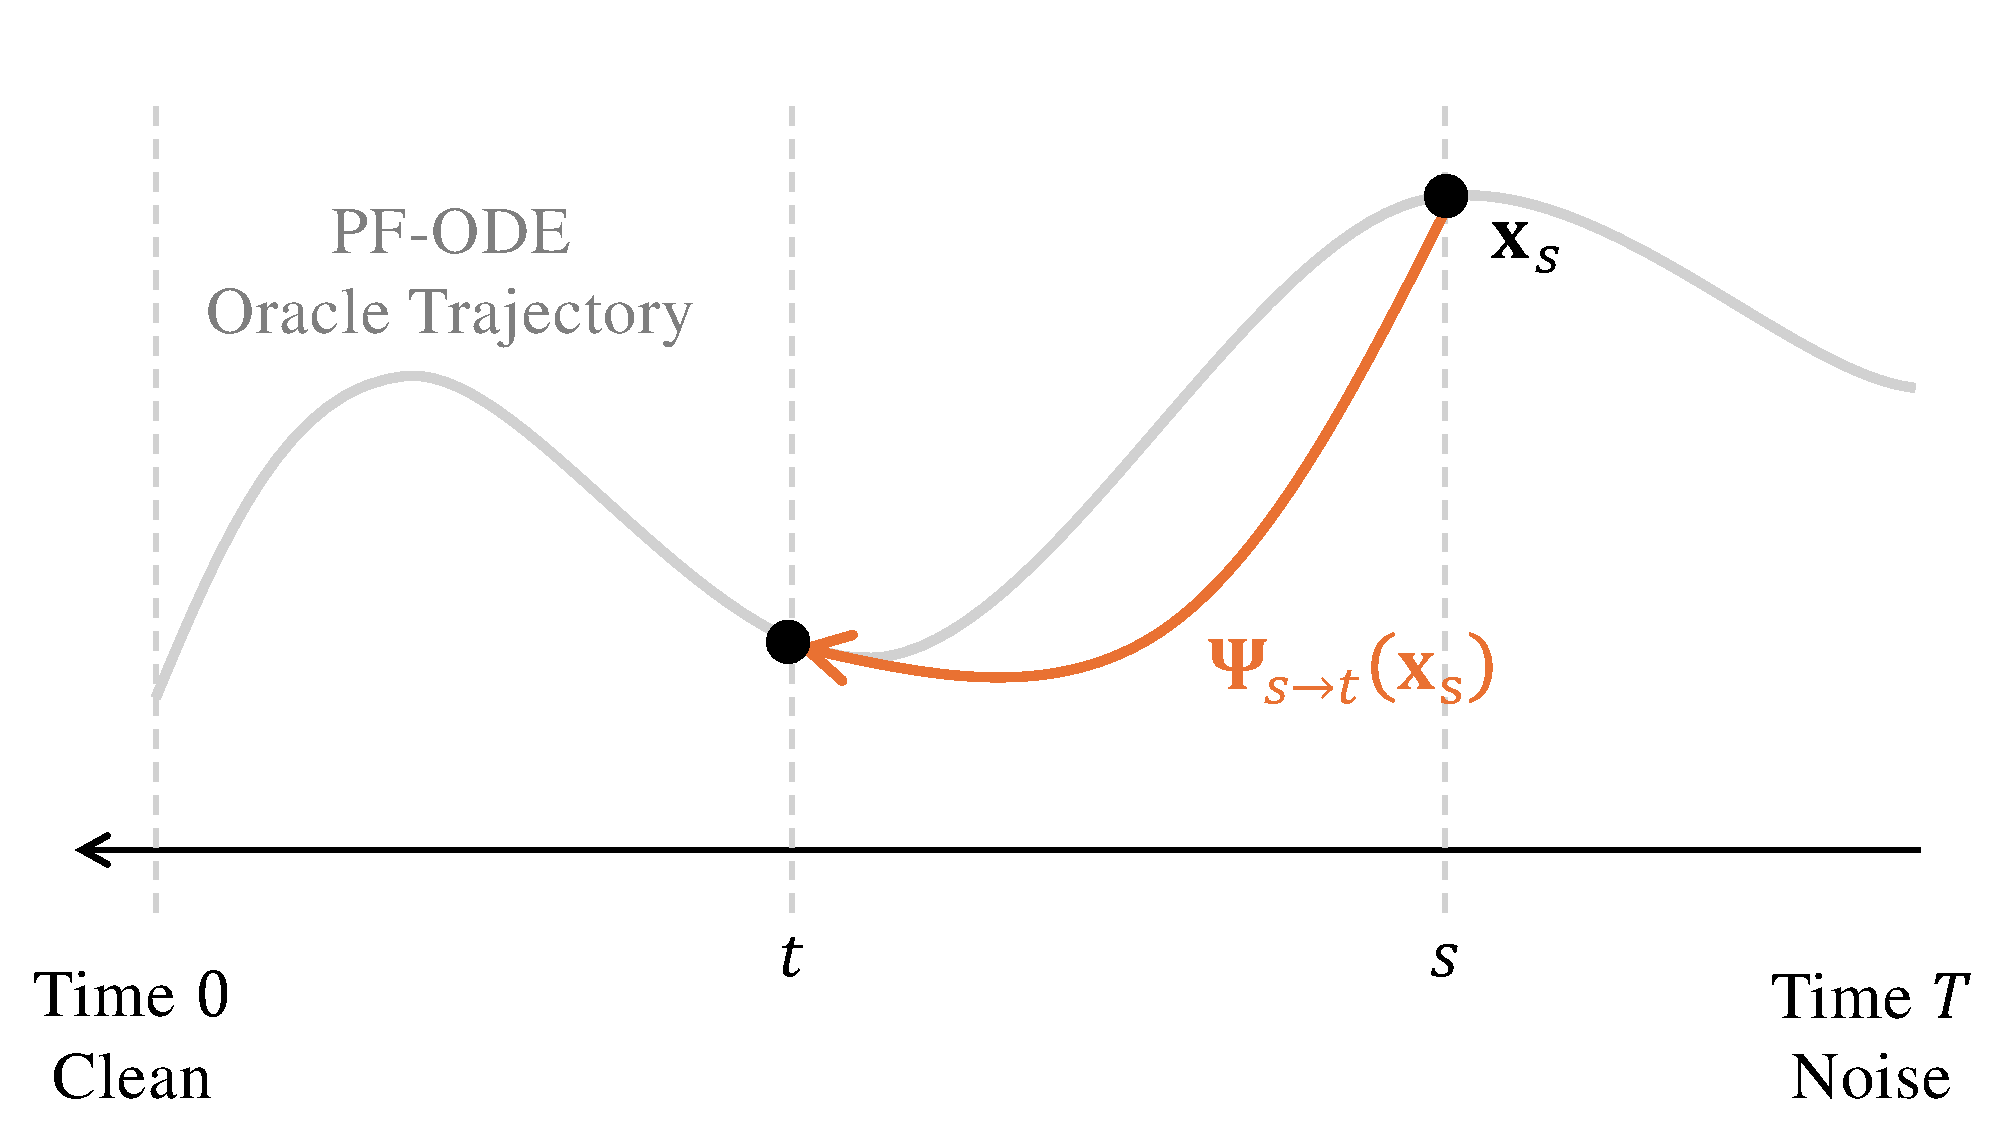
\includegraphics[width=0.9\linewidth]{Images/PartD/flow-map.pdf}
    \caption{\textbfs{流映射的示意图。} 从任意时刻 $s$ 的任意状态 $\rvx_s$ 出发，
流映射 $\bPsi_{s \to t}$ 将其输运到同一 PF-ODE oracle 轨迹上时刻 $t$ 的对应点。\figcredit{由作者绘制。}}
    \label{fig:flow-map-illustration}
\end{figure}


本章围绕一个目标来发展实现该目标的方法，该目标同样支撑着蒸馏，并为流映射的各类公式提供统一视角~\citep{boffi2024flow,hu2025cmt}：
\begin{mdframed}
\begin{equation}\tag{\ref*{eq:general-cm-loss}}\label{eq:general-cm-loss:rep}
  \mathcal{L}_{\mathrm{oracle}}(\btheta)
  := \mathbb{E}_{s,t}\,\mathbb{E}_{\rvx_s \sim p_s}\Big[
     w(s,t)  d\big(\rmG_\btheta(\rvx_s,s,t),  \bPsi_{s\to t}(\rvx_s)\big)
  \Big].
\end{equation}
\end{mdframed}


% Optional: do not consume a new equation number
\addtocounter{equation}{-1}
这里 $s,t$ 从某个时间分布（例如均匀分布）中采样，
$w(s,t) \ge 0$ 为时间对 $(s,t)$ 赋予权重，$d(\cdot,\cdot)$
是某种差异度量，例如 $\ell_2$ 范数的平方。oracle 流映射
$\bPsi_{s\to t}$ 表示这样一种理想变换：取时刻 $s$ 的状态
$\rvx_s$ 并将其直接输运到时刻 $t$：
\[
\bPsi_{s\to t}(\rvx_s) = \rvx_s + \int_s^t \rvv^*(\rvx_u,u)\,\mathrm{d}u,
\]
其中 oracle 漂移项为
\[
\rvv^*(\rvx_u,u) = \E \left[\alpha_u'\rvx_0+ \sigma_u'\beps | \rvx_u\right],
\]
其他等价的参数化也是可行的（见\Cref{ch:all-equivalent}），常见选择包括 $\rvx$-预测和 $\rvv$-预测形式。

在 oracle 损失的最优点处，学习到的模型能够精确恢复真实流映射：
\[
\rmG^*(\rvx_s, s, t) = \bPsi_{s\to t}(\rvx_s), \quad \text{对所有 }\, s,t, \text{ 以及 }\, \rvx_s \sim p_s.
\]


由于流映射 $\bPsi_{s\to t}$ 无法写成闭式，因此必须对其进行近似。
一种选择（已在\Cref{ch:distillation}中讨论）是依赖预训练扩散模型。
或者，正如本章将展示的，可以引入新的、更易处理的代理目标。
为清晰起见，现有方法大致可以根据训练过程是否在循环中查询教师而分类为：
\emph{蒸馏}（显式调用教师模型）和
\emph{从零开始训练}（通过构造自包含的代理目标来避免教师调用）。



基于这一有原则的目标，我们现在转向学习流映射模型的系统性方法，
旨在发展出既实用、又能使生成结果更准确地反映真实数据分布且计算高效的方法。
我们首先对这一范式进行高层次介绍。
\paragraph{特殊流映射：一致性函数。}
\emph{一致性模型}~\citep{song2023consistency} 是流映射学习最早期的开创性方法之一。
它们学习一个少步去噪器 $\rvf_\btheta(\cdot,s)$，用以近似指向原点的流映射这一特殊情形：
\[
\bPsi_{s\to 0}(\cdot), \qquad s \in (0,T].
\]
其核心思想是：每个带噪样本 $\rvx_s$ 都应被映射回其轨迹终点的干净数据点 $\rvx_0$。
形式上，CM 系列~\citep{song2023consistency,songimproved,geng2024consistency,lu2024simplifying} 的 oracle 训练目标为
\begin{align}\label{eq:oracle-cm}
    \mathcal{L}_{\methodl{oracle}{CM}}(\btheta) 
    := \E_{s} \E_{\rvx_s\sim p_s} \left[ w(s)  d \left(\rvf_\btheta(\rvx_s,s), \bPsi_{s\to 0}(\rvx_s)\right)\right].
\end{align}




然而，实践中 oracle $\bPsi_{s\to 0}(\rvx_s)$ 是不可得的。因此它被一个取自同一轨迹上稍早一步 $\bPsi_{s\to s-\Delta s}(\rvx_s)$ 的\emph{停梯度}目标（记为 $\rvf_{\btheta^-}$）所替代：
\[
\bPsi_{s\to 0}(\rvx_s) \approx \rvf_{\btheta^-} \left(\bPsi_{s\to s-\Delta s}(\rvx_s),\,s-\Delta s\right), \quad \Delta s > 0,
\]
其中 $\bPsi_{s\to s-\Delta s}(\rvx_s)$ 本身也必须被近似。有两种
实用的策略：(i) \emph{蒸馏}，依赖预训练扩散模型；(ii) \emph{从零开始训练}，
在无教师引导的情况下使用单点估计。

% \begin{itemize}
%     \item \textbfs{Distillation:} use a one-step solver applied to a pre-trained diffusion model. This approach is called \emph{Consistency Distillation (CD)}.
%     \item \textbfs{From Scratch:} use the analytic one-point estimate
%     \[
%       \rvx_{s-\Delta s} = \alpha_{s-\Delta s}\,\rvx_0 + \sigma_{s-\Delta s}\,\beps,
%     \]
%     with the same $(\rvx_0,\beps)$ as in $\rvx_s = \alpha_s \rvx_0 + \sigma_s \beps$. This approach is called \emph{Consistency Training (CT)}.
% \end{itemize} 


\paragraph{一般流映射。} 两种代表性方法是\emph{一致性轨迹模型}（CTM）和\emph{均值流}（MF）。
\subparagraph{一致性轨迹模型。} \emph{一致性轨迹模型}（CTM）\\~\citep{kim2023consistency} 是首个学习任意起始和终止时刻的一般流映射 $\bPsi_{s\to t}$ 的工作，可以看作是\Cref{eq:general-cm-loss:rep}统一目标下的一个具体实例。CTM 采用受 Euler 启发的参数化，将 oracle 流映射表示为
\begin{align*}
\bPsi_{s\to t}(\rvx_s)
:= \rvx_s + \int_s^t \rvv^*(\rvx_u,u)\diff u 
= \frac{t}{s} \rvx_s
+ \frac{s-t}{s}
\underbrace{\Big[\rvx_s + \frac{s}{s-t} \int_s^t \rvv^*(\rvx_u,u) \diff u\Big]}_{\approx~\rvg_{\btheta}},
\end{align*}
这启发了如下神经参数化
\begin{align}\label{eq:ctm_para_1}
\rmG_{\btheta}(\rvx_s,s,t)
:= \frac{t}{s}\,\rvx_s + \frac{s-t}{s}\,\rvg_\btheta(\rvx_s,s,t),
\end{align}
其中 $\rvg_\btheta$ 是一个神经网络，训练使其满足 $\bPsi_{s\to t}(\rvx_s)\approx \rmG_{\btheta}(\rvx_s,s,t)$。

由于 oracle $\bPsi_{s\to t}(\rvx_s)$ 不可达，CTM 对在中间时刻 $u$ 处求值的\emph{停梯度}目标进行训练：
\[
\bPsi_{s\to t}(\rvx_s)
 \approx
\rmG_{\btheta^-} \big(\bPsi_{s\to u}(\rvx_s),\,u,\,t\big),
\qquad u\in[t,s],
\]
其中中间状态 $\bPsi_{s\to u}(\rvx_s)$ 以两种方式之一进行近似：
(i) \emph{蒸馏}，使用对预训练扩散教师施加的少步求解器；或
(ii) \emph{从零开始训练}，直接通过 $\rmG_\btheta$ 参数化构造自诱导教师。


\subparagraph{均值流。}
均值流（MF）~\citep{geng2025mean} 建立在流匹配之上，对区间 $[t,s]$（$t\le s$）上的\emph{平均漂移}进行建模：
\[
\rvh_{\btheta}(\rvx_s,s,t)
 \approx 
\rvh^*(\rvx_s,s,t)
:= \frac{1}{\,t-s\,}\int_s^t \rvv^*(\rvx_u,u)\,\diff u,
\]
同样与\Cref{eq:general-cm-loss:rep}对齐。
对恒等式
\[
(t-s)\,\rvh^*(\rvx_s,s,t)  =  \int_s^t \rvv^*(\rvx_u,u)\,\diff u
\]
关于 $s$ 求导，得到一个自指关系，由此启发 MF 目标
\[
\mathcal{L}_{\mathrm{MF}}(\btheta)
:= \E_s\,\E_{\rvx_s\sim p_s} \Big[w(s)\,\big\|
\rvh_{\btheta}(\rvx_s,s,t)-\rvh_{\btheta^-}^{\mathrm{tgt}}(\rvx_s,s,t)
\big\|_2^2\Big],
\]
其停梯度目标为
\[
\rvh_{\btheta^-}^{\mathrm{tgt}}(\rvx_s,s,t)
:= \rvv^*(\rvx_s,s)  -  (s-t) \left(\rvv^*(\rvx_s,s)\,\partial_\rvx \rvh_{\btheta^-} + \partial_s \rvh_{\btheta^-}\right).
\]
实践中，oracle 速度 $\rvv^*(\rvx_s,s)$ 也必须被近似。
两种常见策略为：(i) \emph{蒸馏}，利用经流匹配训练的预训练扩散模型；或 (ii) \emph{从零开始训练}，
使用由前向加噪过程 $\rvx_s = \alpha_s \rvx_0+\sigma_s \beps$ 导出的单点条件速度
$\alpha'_s\,\rvx_0+\sigma'_s\,\beps$。



\subparagraph{CTM 与 MF 之间的关系。}
CTM 与 MF 近似的是同一路径积分，但对其参数化了不同的代理目标：
\begin{align*}
\bPsi_{s\to t}(\rvx_s)
&:= \rvx_s  +  \int_s^t \rvv^*(\rvx_u,u)\,\diff u
\\[2pt]
&= \frac{t}{s}\,\rvx_s
 +  \frac{s-t}{s}\,
\underbrace{\Big[\rvx_s + \frac{s}{\,s-t\,} \int_s^t \rvv^*(\rvx_u,u)\,\diff u\Big]}_{\approx~\rvg_{\btheta} }
\\[4pt]
&= \rvx_s  +  (t-s)\,
\underbrace{\Big[\frac{1}{\,t-s\,} \int_s^t \rvv^*(\rvx_u,u)\,\diff u\Big]}_{\approx~\rvh_{\btheta} }.
\end{align*}
换言之，CTM 通过 $\rvg_\btheta$ 学习\emph{斜率位移}，而 MF 学习\emph{平均漂移} $\rvh_\btheta$；两者都是近似定义 $\bPsi_{s\to t}$ 的同一积分的一致方式。


\paragraph{接下来的内容。}
我们从 CM 系列开始，它关注特定的流映射
$\bPsi_{s\to 0}$。这部分既包括其在\Cref{sec:discrete-cm}中的离散时间起源，
也包括在\Cref{sec:conti-cm}中的连续时间扩展。然后我们转向一般流映射，
详细讨论两个关键代表 CTM 和 MF。它们的参数化、训练策略和实用近似分别在
\Cref{sec:CTM}和\Cref{sec:MF}中介绍。

我们指出，\Cref{sec:edm}中介绍的\emph{阐释扩散模型}（EDM）为
设计 $\rvx$-预测模型的网络参数化提供了系统性指南，并在经验上表现出色。
虽然本节可视为可选，但 EDM 公式是 CM 类模型的重要基础。


为便于后续论述清晰，我们不严格遵循这些方法出现的时间顺序。
相反，我们按概念关系来组织讨论。
不过，为承认原创性并尊重时间顺序，我们在\Cref{fig:timeline}中给出历史时间线。




%%%%%%%%%%%%%%%%%%%%%%%%


\clearpage
\newpage


\section{特殊流映射：离散时间一致性模型}\label{sec:discrete-cm}

\paragraph{流映射的一个重要原理：半群性质。}
\begin{figure}[th!]
    \centering
    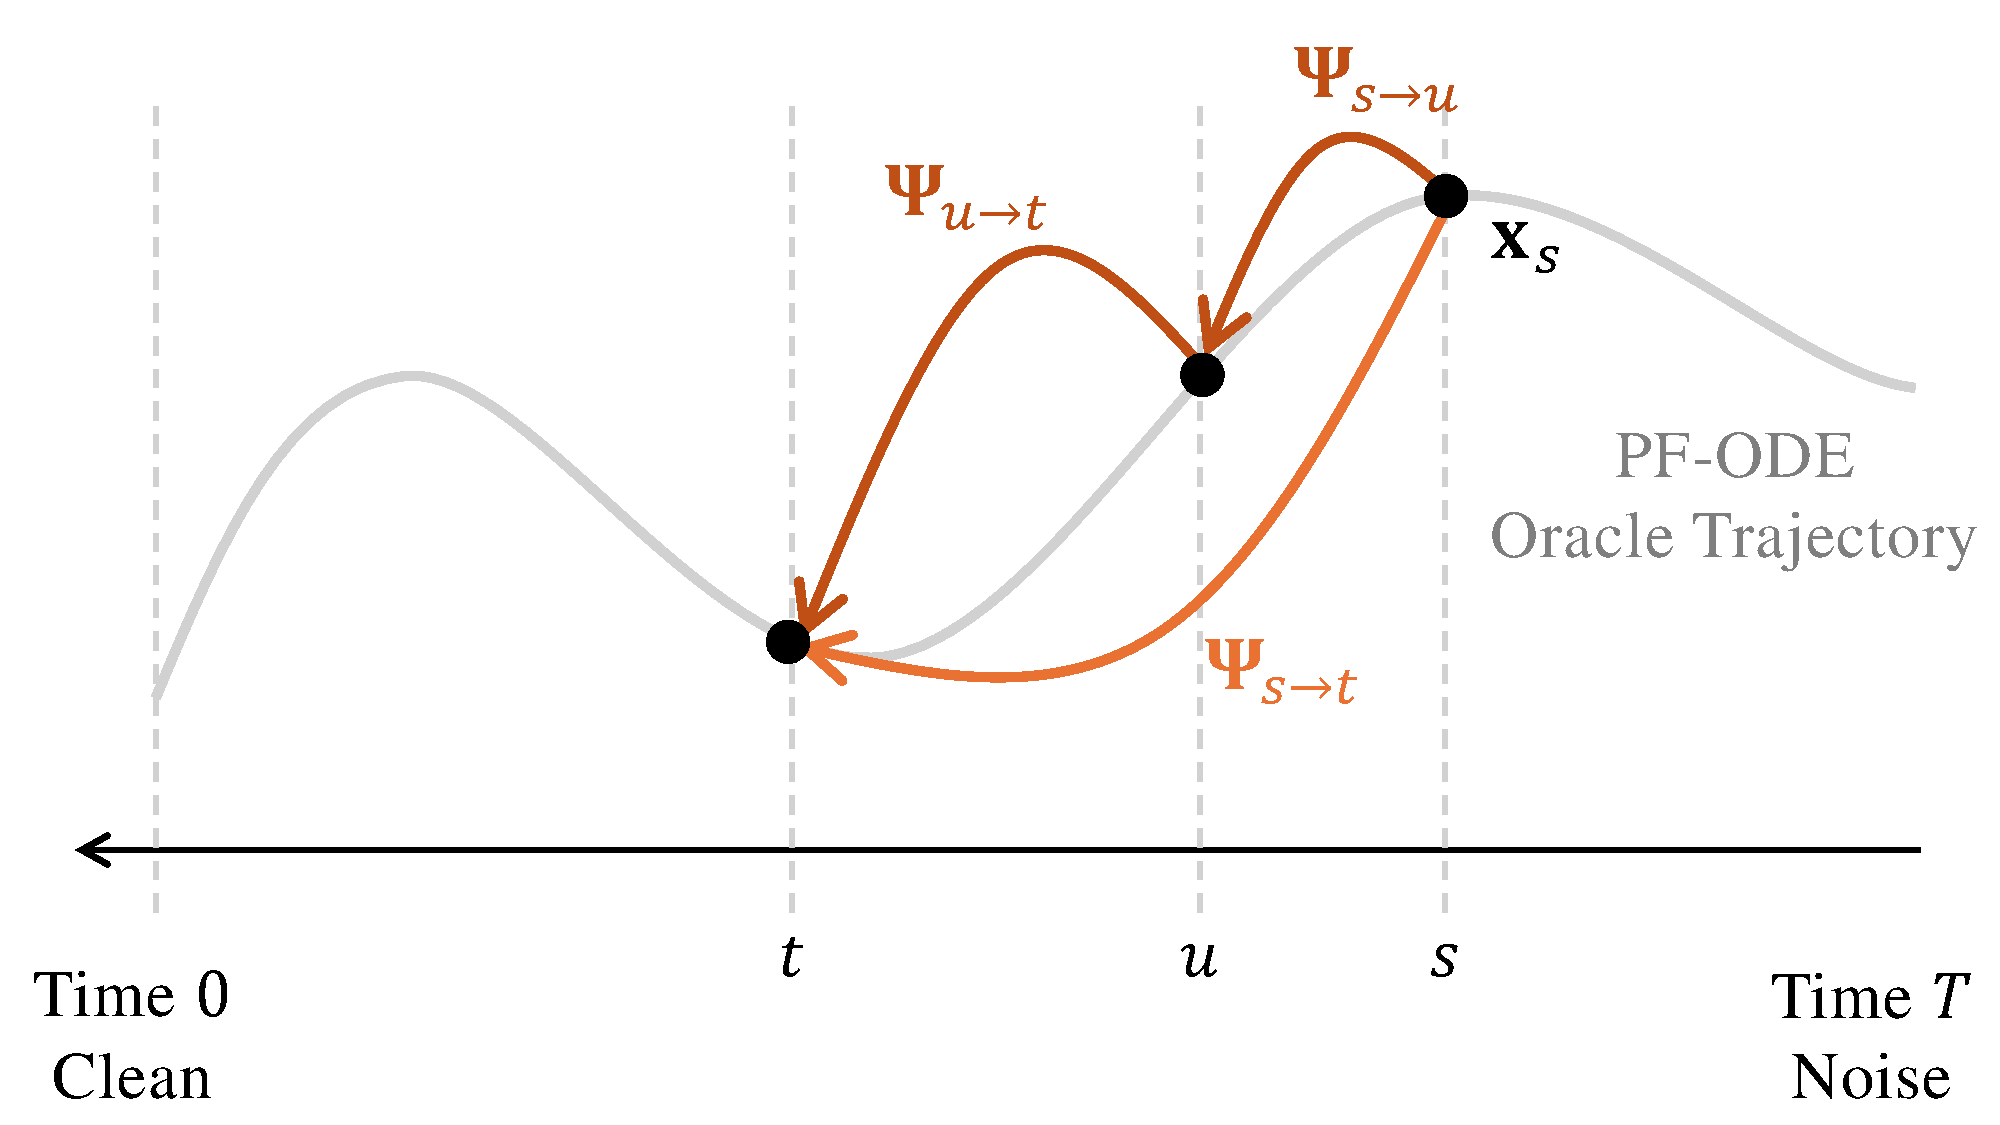
\includegraphics[width=0.9\linewidth]{Images/PartD/semigroup.pdf}
    \caption{\textbfs{流映射半群性质的示意图。}
该性质表明，先从 $s$ 转移到 $u$，再从 $u$ 转移到 $t$，
等价于直接从 $s$ 转移到 $t$。
\figcredit{由作者绘制。}}
    \label{fig:semigroup}
\end{figure}


一致性模型（在\Cref{sec:discrete-cm,sec:conti-cm}中介绍）及其推广——一致性轨迹模型（\Cref{sec:CTM}），都通过利用流映射的一种关键数学结构来定义其回归目标。
这种结构就是基本的\emph{半群性质}：
\begin{mdframed}
   \begin{align}\label{eq:semi-group}
       \bPsi_{u\to t}\circ \bPsi_{s\to u}=\bPsi_{s\to t},
       \,\,\,
       \bPsi_{s\to s}=\rmI, \quad \text{对所有 }\, s, u, t \in [0,T].
   \end{align} 
\end{mdframed}
直观上，这意味着如果我们先将状态从 $s$ 演化到 $u$（通过 $\bPsi_{s\rightarrow u}$），再从 $u$ 演化到 $t$（通过 $\bPsi_{u\rightarrow t}$），最终到达的点与直接从 $s$ 演化到 $t$ 完全相同。
这不过是 ODE 求解的基本原理\footnote{半群性质源自 ODE 初值问题唯一性定理（见\Cref{app:de}）。}：一旦流的起点给定，其未来演化就被完全确定，并遵循唯一明确的路径。无论我们用一大步沿此路径前进，还是将其划分为更小的区间，我们仍然沿同一轨迹移动并到达相同的终点。

为了进一步建立对半群性质的直觉，考虑 PF-ODE 的解轨迹 $\{\rvx(s)\}_{s \in [0,T]}$
\begin{align*}
    \frac{\diff \rvx(\tau)}{\diff \tau} = \rvv^*(\rvx(\tau), \tau),
\end{align*}
其在时刻 $T$ 处给定固定初值 $\rvx(T)$，沿时间向后求解。
若我们将终点时刻固定为 $t=0$，相应的流映射可以更简单地写为
\[
\rvf^*(\cdot, s) := \bPsi_{s\to 0}(\cdot),
\]
称之为\emph{一致性函数}。
按构造，该函数直接从\Cref{eq:semi-group}在 $t=0$ 时的半群恒等式继承了几条基本性质：

\begin{enumerate}
    \item[(i)] \textbfs{全局一致性：}轨迹上的每一点都映射到相同的干净终点，
    \[
       \rvf^*(\rvx(s), s) = \rvx(0), \quad \text{对所有 }\, s \in [0,T].
    \]
    这是因为
\begin{align*}
\rvf^*(\rvx(s),s)
&= \bPsi_{s\to 0}\big(\bPsi_{0\to s}(\rvx(0))\big)
= \big(\bPsi_{s\to 0}\circ \bPsi_{0\to s}\big)(\rvx(0))
\\&= \bPsi_{0\to 0}(\rvx(0))
= \rvx(0).
\end{align*}
    \item[(ii)] \textbfs{自一致性：}同一轨迹上任意两点必须给出相同的输出，
    \begin{align}\label{eq:cm-self-consistency}
       \rvf^*(\rvx(s), s) = \rvf^*(\rvx(u), u), \quad \text{对所有 }\, s, u \in [0,T].
    \end{align}
    这是对半群恒等式的直接重释：$\Psi_{s\rightarrow 0}\circ\Psi_{0\rightarrow s}=\Psi_{u\rightarrow 0}\circ\Psi_{0\rightarrow u}$。
    \item[(iii)] \textbfs{局部一致性：}沿轨迹求值时，一致性函数关于 $s$ 不变，
    \begin{align}\label{eq:cm-diff}
        \frac{\diff}{\diff s}\,\rvf^*(\rvx(s),s) = 0,
        \qquad \rvf^*(\rvx(0),0) = \rvx(0).
    \end{align}
这由全局一致性得到，后者指出 $\rvf^*(\rvx(s), s)$ 沿轨迹不随 $s$ 改变。
\end{enumerate}
这三条性质彼此等价。每一条都表明：沿任意解轨迹 $s\mapsto \rvx(s)$，
流到原点/一致性映射 $\rvf^*(\rvx(s),s)=\bPsi_{s\to 0}(\rvx(s))$
都给出相同的终点 $\rvx(0)$，与起始时刻无关。


\paragraph{一致性模型的目标。}
CM 旨在训练一个神经网络
$\rvf_{\bm{\theta}} \colon \mathbb{R}^D \times [0,T] \to \mathbb{R}^D$
来近似特殊流映射 $\bPsi_{s\to 0}$，即一致性函数\footnote{ODE 的一致性函数概念可推广到 SDE 上满足如下条件的函数
$\rvf(\rvx,t)$：使 $\rvf(\rvx_t,t)$ 成为关于 SDE 自然 $\sigma$-代数流的（局部）鞅，即
\[
\E[\rvf(\rvx_t,t)|\rvx_s]=\rvf(\rvx_s,s),\quad\text{对所有 }\quad t\ge s.
\]
这一推广在\citep{daras2023consistent,lai2023fp}中被提出/观察到，
理论上的联系总结于\citep{lai2023equivalence}。}。
其核心思想是在 PF-ODE 的多条轨迹上强制执行半群性质，确保同一数据点的不同带噪版本一致地映射回相同的干净原点（更确切地说，这对应于\Cref{eq:semi-group}中 $t=0$ 且 $u=s-\Delta s$ 的特殊情形）。

然而，实现这一目标有多种方式。
其选择取决于是否有可用的预训练扩散模型，以及训练是在离散时间还是连续时间体系下进行。
我们先在\Cref{tb:consistency-methods}中概述这些变体，并在\Cref{fig:cd-ct-loss-distill}中示意它们的目标。
随后的几节（\Cref{sec:discrete-cm,sec:conti-cm}）再逐步展开每种方法的细节。

\begin{table}[th]
  \caption{一致性模型的训练目标}
  \small
  \centering
  \resizebox{0.76\textwidth}{!}{
  \begin{tabular}{ccc}
     \toprule
     & \textbfs{蒸馏} & \textbfs{从零开始} \\
     \midrule
     \textbfs{离散时间} & \Cref{eq:cd-discrete-approx-N} & \Cref{eq:ct-discrete-approx-N} \\
     \textbfs{连续时间} & \Cref{eq:cd-continuous-time}  & \Cref{eq:ct-continuous-time} \\
     \bottomrule
  \end{tabular}
  }
  \label{tb:consistency-methods}
\end{table} 




\subsection{学习一致性函数的离散时间近似}\label{subsec:approx-cm}

原则上，可以通过最小化 oracle 损失\Cref{eq:oracle-cm}来学习一致性函数：
\[
    \mathcal{L}_{\methodl{oracle}{CM}}(\btheta)
    := \E_{s} \E_{\rvx_s\sim p_s} \left[ w(s)  d \left(\rvf_\btheta(\rvx_s,s), \bPsi_{s\to 0}(\rvx_s)\right)\right].
\]
该目标强制每个带噪样本 $\rvx_s$ 都被映射回其干净终点 $\bPsi_{s\to 0}(\rvx_s)$。

挑战在于 oracle 映射 $\bPsi_{s\to 0}(\rvx_s)$ 在实践中不可得。
为克服这一点，\citet{song2023consistency} 利用\emph{半群性质}：同一 PF-ODE 轨迹上的任意带噪状态及其相邻步骤必然映射到相同的干净终点。
具体地，oracle 目标被轨迹上稍早一点处的\emph{停梯度}目标所替代：
\begin{align*}
    \bPsi_{s\to 0}(\rvx_s)
    &= \bPsi_{s-\Delta s \to 0} \left(\bPsi_{s\to s-\Delta s}(\rvx_s)\right) \\
    &\approx \rvf_{\btheta^-} \left(\bPsi_{s\to s-\Delta s}(\rvx_s),\,s-\Delta s\right),
    \qquad \Delta s > 0,
\end{align*}
其中 $\bm{\theta}^-$ 是停梯度算子下的参数。
进一步的困难在于，中间状态 $\bPsi_{s\to s-\Delta s}(\rvx_s)$ 同样没有闭式，必须自身被近似。
已提出两种实用体系：

\paragraph{有预训练扩散模型（一致性蒸馏）。}
假设我们可以访问一个预训练的扩散模型。
一致性蒸馏（CD）利用教师模型，通过仅模拟单步反向 ODE 步骤来近似中间状态 $\bPsi_{s\to s-\Delta s}(\rvx_s)$：
\[
 \bPsi_{s\to s-\Delta s}(\rvx_s)  \approx  \mathtt{Solver}_{s \to s-\Delta s}(\rvx_s).
\]

更具体地说，预训练扩散模型提供了得分函数的估计
$\rvs_{\bm{\phi}^\times}(\rvx_s, s) \approx \nabla_{\rvx_s}\log p_s(\rvx_s)$。
利用它，可以从 $\rvx_s$ 执行一步 DDIM 更新，得到 $s' = s-\Delta s$ 处状态的近似：
\begin{align*}
    \bPsi_{s\to s-\Delta s}(\rvx_s) 
    &\approx \frac{\alpha_{s'}}{\alpha_s}\,\rvx_s 
    + \sigma_s^2 \left( \frac{\alpha_{s'}}{\alpha_s} - \frac{\sigma_{s'}}{\sigma_s} \right)\nabla_{\rvx_s}\log p_s(\rvx_s) \\
    &\approx \frac{\alpha_{s'}}{\alpha_s}\,\rvx_s 
    + \sigma_s^2 \left( \frac{\alpha_{s'}}{\alpha_s} - \frac{\sigma_{s'}}{\sigma_s} \right)\rvs_{\bm{\phi}^\times}(\rvx_s, s) \\
    &:= \tilde{\rvx}_{s'}^{\bm{\phi}^\times}.
\end{align*}

将此构造与停梯度目标结合，便得到 oracle 损失 $\mathcal{L}_{\methodl{oracle}{CM}}(\btheta)$ 的实用\emph{离散时间}代理。
形式上，在划分 $0 = s_1 < s_2 < \cdots < s_N = T$ 上，CD 的训练目标为
\begin{mdframed}
\begin{align}\label{eq:cd-discrete-approx-N}
    \mathcal{L}_{\text{CD}}^N(\bm{\theta}, \bm{\theta}^-; \bm{\phi}^\times)
    := \E_{\rvx_0, \beps, i} \Big[\, \omega(s_i)\,
    d\big(\rvf_{\bm{\theta}}(\rvx_{s_{i+1}}, s_{i+1}),\,
          \rvf_{\bm{\theta}^-}(\tilde{\rvx}_{s_i}^{\bm{\phi}^\times}, s_i)\big)\Big].
\end{align}
\end{mdframed}
这里，$\omega(\cdot)$ 是一个时间相关的权重，$d(\cdot,\cdot)$ 是距离度量，$\bm{\theta}^-$ 表示停梯度参数，用于防止塌缩到平凡解（例如常数预测）。



\paragraph{没有预训练扩散模型（一致性训练）。}
当没有可用的预训练扩散模型时，oracle 得分 $\nabla_{\rvx}\log p_s(\rvx_s)$ 仍然可以通过简单的单点近似直接估计（尽管方差较高）。
回忆它具有条件期望形式：
\begin{align*}
    \nabla_{\rvx_s} \log p_s(\rvx_s)
    &= \E_{\rvx_0 \sim p(\rvx_0|\rvx_s)} \left[ \nabla_{\rvx_s}\log p(\rvx_s|\rvx_0) \right] \\
    &= \E_{\rvx_0 \sim p(\rvx_0|\rvx_s)} \left[ -\frac{\rvx_s - \alpha_s \rvx_0}{\sigma_s^2} \right].
\end{align*}
上述恒等式暗示了一个简单的单样本估计器。
若 $\rvx_s$ 是由配对样本 $(\rvx_0,\beps)$ 通过 $\rvx_s = \alpha_s \rvx_0 + \sigma_s \beps$ 得到的，则
\[
\widehat{\nabla_{\rvx}\log p_s}(\rvx_s)
:=-\frac{\boldsymbol\epsilon}{\sigma_s}
=-\frac{\rvx_s-\alpha_s \rvx_0}{\sigma_s^2}
\]
作为 $\rvx_s$ 处得分的一个\emph{无偏}估计器（在给定 $p(\rvx_0|\rvx_s)$ 时条件无偏）。它恰好对应于去噪得分匹配中用作回归目标的\emph{条件得分}。



将该估计代入从 $s$ 到 $s' = s-\Delta s$ 的 DDIM 一步更新（见\Cref{eq:ddim-update-all}）得到
\begin{align}\label{eq:one-pt-score}
\begin{aligned}
    \bPsi_{s\to s'}(\rvx_s)
&\approx
\frac{\alpha_{s'}}{\alpha_s}\,\rvx_s
+ \sigma_s^2 \left(\frac{\alpha_{s'}}{\alpha_s}-\frac{\sigma_{s'}}{\sigma_s}\right)\nabla_{\rvx_s}\log p_s(\rvx_s) && \text{(DDIM)}
\\
&\approx
\frac{\alpha_{s'}}{\alpha_s}\,\rvx_s
+ \sigma_s^2 \left(\frac{\alpha_{s'}}{\alpha_s}-\frac{\sigma_{s'}}{\sigma_s}\right)\widehat{\nabla_{\rvx_s}\log p_s}(\rvx_s) && \text{(单点得分)}
\\
&=
\frac{\alpha_{s'}}{\alpha_s}\,\rvx_s
-\left(\frac{\alpha_{s'}}{\alpha_s}-\frac{\sigma_{s'}}{\sigma_s}\right)(\rvx_s-\alpha_s\rvx_0)
\\
&= \alpha_{s'}\rvx_0+\sigma_{s'}\beps,
\end{aligned}
\end{align}
其中\footnote{最后一个恒等式由前向加噪过程 $\rvx_s=\alpha_s \rvx_0+\sigma_s \beps$ 经初等代数运算直接得到。}
$\rvx_0$ 是相同的数据样本，$\beps$ 是用于构造 $\rvx_s$ 的相同高斯噪声。


由此得到 oracle 目标 $\mathcal{L}_{\methodl{oracle}{CM}}$ 的一个无需教师的离散时间代理，写作
\begin{mdframed}
\begin{align}\label{eq:ct-discrete-approx-N}
    \mathcal{L}_{\text{CT}}^N(\bm{\theta}, \bm{\theta}^-) 
    := \E_{\rvx_0, \beps, i} \left[ 
       \omega(s_i)\, d \left(\rvf_{\bm{\theta}}(\rvx_{s_{i+1}}, s_{i+1}),\, 
       \rvf_{\bm{\theta}^-}(\rvx_{s_i}, s_i)\right)
    \right],
\end{align}
\end{mdframed}
with $\rvx_{s_i} = \alpha_{s_i}\rvx_0 + \sigma_{s_i}\beps$ and $\rvx_{s_{i+1}} = \alpha_{s_{i+1}}\rvx_0 + \sigma_{s_{i+1}}\beps$.

直接用 $\alpha_{s'}\rvx_0+\sigma_{s'}\beps$ 作为 $\bPsi_{s\to s'}(\rvx_s)$ 的近似而不取期望，会引入较高方差\footnote{单点（条件）得分估计 $\widehat{\nabla_{\rvx}\log}p_s(\rvx_s)$ 可视为一个单样本蒙特卡洛估计器，它在给定 $\rvx_s$ 时是\emph{条件无偏}的：在（通常难以处理的）干净后验 $p(\cdot|\rvx_s)$ 上对该估计器求平均可恢复真实得分
\[
\nabla_{\rvx_s}\log p_s(\rvx_s)
= \E_{\rvx_0\sim p(\cdot|\rvx_s)}
 \left[\widehat{\nabla_{\rvx}\log}p_s(\rvx_s)\right].
\]}。
然而，回忆去噪得分匹配中的类似情形（见\Cref{sec:conditional-trick}），其中单个条件得分样本作为训练目标，但一旦在损失中对 $\rvx_0,\beps$ 取平均，便成为无偏的。
同理，$\mathcal{L}_{\mathrm{CT}}^N$ 中对 $\rvx_0$ 和 $\beps$ 的期望会平均掉这种采样噪声，得到无偏的损失级别近似。下面的定理将这种期望级别的论证形式化，以证明单点估计器的合理性。

% The one-point (conditional) score estimate $\widehat{\nabla_{\rvx}\log}p_s(\rvx_s)$ can be viewed as a one-sample Monte Carlo estimator, which is \emph{conditionally unbiased} given $\rvx_s$: averaging this estimator over the (generally intractable) clean posterior $p(\cdot|\rvx_s)$ recovers the true score as
% \[
% \nabla_{\rvx_s}\log p_s(\rvx_s)
% = \E_{\rvx_0\sim p(\cdot|\rvx_s)}
%  \left[\widehat{\nabla_{\rvx}\log}p_s(\rvx_s)\right].
% \]
% If one uses $\alpha_{s'}\rvx_0+\sigma_{s'}\beps$ directly as an approximation of $\bPsi_{s\to s'}(\rvx_s)$ without expectation generally yields high variance. 
% However, after taking the full expectation in the loss (Theorem~\ref{thm:ct-cm}), this one-sample estimator remains unbiased; hence, the one-point score approximation is justified at the loss level.
% In this sense, the update below serves as a practical approximation to the DDIM step computed with an oracle score.
% The following theorem formalizes this expectation-level justification of the one-point estimator.

% and hence,
% \begin{align}
% \begin{aligned}
%     \bPsi_{s\to s'}(\rvx_s)
% &\approx
% \frac{\alpha_{s'}}{\alpha_s}\,\rvx_s 
% + \sigma_s^2 \left(\frac{\alpha_{s'}}{\alpha_s}-\frac{\sigma_{s'}}{\sigma_s}\right)\nabla_{\rvx_s}\log p_s(\rvx_s) && \text{(DDIM)}
% \\
% &=
% \frac{\alpha_{s'}}{\alpha_s}\,\rvx_s 
% + \sigma_s^2 \left(\frac{\alpha_{s'}}{\alpha_s}-\frac{\sigma_{s'}}{\sigma_s}\right) \E_{\rvx_0\sim p(\cdot|\rvx_s)}
%  \left[\widehat{\nabla_{\rvx}\log}p_s(\rvx_s)\right] 
% \\
% &=
% \frac{\alpha_{s'}}{\alpha_s}\,\rvx_s 
% -\left(\frac{\alpha_{s'}}{\alpha_s}-\frac{\sigma_{s'}}{\sigma_s}\right)(\rvx_s-\alpha_s\rvx_0)
% \\
% &=  \E_{\rvx_0\sim p(\cdot|\rvx_s)}
%  \left[\rvx_0+\sigma_{s'}\beps\right]\alpha_{s'}=:\hat\rvx_{s'}, 
% \end{aligned}
% \end{align}




\thmp{CM-CT 在误差 $\mathcal{O}(\Delta s^2)$ 内的等价性}{ct-cm}{
令 $s' := s - \Delta s$，并定义
\begin{align*}
\mathcal{L}_{\mathrm{CM}}(\btheta,\btheta^-)
&:= \E_{s,\rvx_0,\beps} \big[w(s)\,d\big(\rvf_{\btheta}(\rvx_s,s), \rvf_{\btheta^-}(\rvx_{s'}^{\mathrm{DDIM}},s')\big)\big],\\
\mathcal{L}_{\mathrm{CT}}(\btheta,\btheta^-)
&:= \E_{s,\rvx_0,\beps} \big[w(s) d\big(\rvf_{\btheta}(\rvx_s,s), \rvf_{\btheta^-}(\rvx_{s'},s')\big)\big],
\end{align*}
其中
\[
\rvx_{s'}^{\mathrm{DDIM}}
:= \frac{\alpha_{s'}}{\alpha_s}\rvx_s
+ \sigma_s^2 \left(\frac{\alpha_{s'}}{\alpha_s}-\frac{\sigma_{s'}}{\sigma_s}\right)\nabla_{\rvx_s}\log p_s(\rvx_s)
\]
是 oracle DDIM 更新。$\rvx_s = \alpha_s\rvx_0 + \sigma_s\beps$ 和 $\rvx_{s'} = \alpha_{s'}\rvx_0 + \sigma_{s'}\beps$
共享同一对 $(\rvx_0,\beps)$，其中
$\rvx_0 \sim p_{\mathrm{data}}$，且
$\beps \sim \mathcal{N}(\bm{0},\rmI)$。
则
\[
\mathcal{L}_{\mathrm{CM}}(\btheta,\btheta^-)
= \mathcal{L}_{\mathrm{CT}}(\btheta,\btheta^-) + \mathcal{O}(\Delta s^2).
\]
}{首先，注意使用 oracle 得分的 DDIM 更新等于条件均值，
\[
\rvx_{s'}^{\mathrm{DDIM}} = \E[\rvx_{s'} | \rvx_s],
\]
这也可在\Cref{eq:one-pt-score}中对 $p(\cdot|\rvx_s)$ 取期望来验证。
接下来，对
\[
d(\rvf_{\btheta}(\rvx_s,s), \rvf_{\btheta^-}(\cdot,s'))
\]
在 $\rvx_{s'}^{\mathrm{DDIM}}=\E[\rvx_{s'}|\rvx_s]$ 处进行 Taylor 展开。Taylor 展开的线性项消失，因为内层期望在 $\rvx_{s'} | \rvx_s$ 上取，满足 $\E[\rvx_{s'}-\rvx_{s'}^{\mathrm{DDIM}}|\rvx_s]=0$。这表明，通过将条件重新参数化为
$\E_{\rvx_0,\beps|\rvx_s}[\cdot]$，其中
$\rvx_{s'}=\alpha_{s'}\rvx_0+\sigma_{s'}\beps$，
使用单点得分的 DDIM 更新对相同 $(\rvx_0,\beps)$ \emph{逐路径}精确恢复
$\rvx_{s'}$，因此内层期望保持不变。剩余项是二次项，即 $\mathcal{O}(\Delta s^2)$，故 $\mathcal{L}_{\mathrm{CT}}=\mathcal{L}_{\mathrm{CM}}+\mathcal{O}(\Delta s^2)$。
详细的推导见\Cref{app-sec:flow-map}。
}


总之，CD 利用教师模型进行初始化和引导，通常能稳定优化并降低方差。相反，一致性训练（CT）不需要预训练模型，因此可以完全从零开始训练。
尽管存在这一差异，CT 仍可作为完全独立的生成模型。


\paragraph{实践考虑。}
在实践中，\citet{song2023consistency} 采用 \citet{karras2022elucidating} 的 EDM 公式（见\Cref{sec:edm}），前向加噪核为
\[
    \rvx_s = \rvx_0 + s \bm{\epsilon},
\]
并使用其中提出的神经网络参数化
（参见\Cref{eq:D-parametrization}）：
\[
    \rvf_{\bm{\theta}}(\rvx, s)
    = c_{\mathrm{skip}}(s) \rvx
      + c_{\mathrm{out}}(s)\,
        \rmF_{\bm{\theta}} \left(c_{\mathrm{in}}(s)\,\rvx,\, c_{\mathrm{noise}}(s)\right),
\]
其中 $\rmF_{\bm{\theta}}$ 是一个神经网络，系数遵循
\Cref{eq:edm-simple-coefficients}。该参数化具有一个重要的边界性质
\[
    \rvf_{\bm{\theta}}(\rvx, 0) = \rvx,
\]
它在时刻零处强制一致性，并确保网络输出在无噪声时与其输入匹配。





% Assume that $\rvf_{\bm{\theta}}$ learns the optimal trajectory defined by the empirical PF-ODE of the teacher model as in \Cref{eq:teacher-pf-ode}. We revisit \Cref{eq:conti-ct-motivation}  when staying on a trajectory $\{\bar\rvx(s)\}_{s\in[0, T]}$ of the empirical ODE: 
% \begin{align*}
%         &\rvf_{\bm{\theta}^*}(\bar\rvx(s), s) \equiv \bar\rvx(0), \quad \text{for all } s\in [0,T]
%         \\
%         \Leftrightarrow~&\left(\nabla_{\rvx} \rvf_{\bm{\theta}^*}\right)(\bar\rvx(s), s) \cdot 
%     \underbrace{\frac{\diff }{\diff s} \bar\rvx(s)}_{\text{ODE velocity}} + 
%     \left(\frac{\partial }{\partial s} \rvf_{\bm{\theta}^*}\right)(\bar\rvx(s), s) \equiv 0\\
%         \Leftrightarrow~&\left(\nabla_{\rvx} \rvf_{\bm{\theta}^*}\right)(\bar\rvx(s), s) \cdot \rvv_{\bm{\phi}^\times}(\bar\rvx(s), s) + \left(\frac{\partial }{\partial s} \rvf_{\bm{\theta}^*}\right)(\bar\rvx(s), s) \equiv 0
%     \end{align*}

\subsection{使用一致性模型采样}\label{subsec:cm-sampling}
一旦一致性模型 $\rvf_{\bm{\theta}^\times}$ 训练完成，无论是连续时间还是离散时间，都可以用于单步或数步生成样本。算法总结于\Cref{alg:cm_sampling}。

\paragraph{单步生成。} 给定从先验分布采样的初始隐变量 $\hat{\rvx}_T$（实践中为 $\mathcal{N}(\bm{0}, T^2\rmI)$），可通过单次函数求值生成干净样本：
\begin{align*}
    \rvf_{\bm{\theta}^\times}(\hat{\rvx}_T, T).
\end{align*}
\paragraph{多步生成。} 给定预设的时刻序列
\[
T>\tau_1 > \tau_2 > \cdots > \tau_{M-1}=0,
\]
从初始噪声 $\hat\rvx_T$ 出发，在较早时刻通过一致性模型交替进行噪声注入和大跨度干净跳转，逐步精炼样本：
\begin{align*}
    \hat\rvx_T \xrightarrow[\text{得到干净样本}]{\text{长跳}} \rvf_{\bm{\theta}^\times}(\hat{\rvx}_T, T)
    \xrightarrow[\text{到层级 $\tau_1$}]{\text{加噪}} \hat\rvx_{\tau_1}
    \xrightarrow[\text{得到干净样本}]{\text{长跳}} \rvf_{\bm{\theta}^\times}(\hat\rvx_{\tau_1}, \tau_1)
    \xrightarrow[\text{到层级 $\tau_2$}]{\text{加噪}} \cdots.
\end{align*}

\begin{algorithm}[thb!]
    {\small
        \caption{CM 的单步或多步生成采样 \label{alg:cm_sampling}}
    \begin{algorithmic}[1]
        \Require 一致性模型 $\rvf_{\bm{\theta}^\times}(\cdot, \cdot)$，时间点序列 $T>\tau_1 > \tau_2 > \cdots > \tau_{M-1}=0$，初始噪声 $\hat{\rvx}_T$
        \If{单步}
            \State $\rvx \leftarrow \rvf_{\bm{\theta}^\times}(\hat{\rvx}_T, T)$
        \Else
            \State $\rvx \leftarrow \rvf_{\bm{\theta}^\times}(\hat{\rvx}_T, T)$
            \For{$m=1$ \textbf{到} $M-1$}
                \State 采样 $\bm{\epsilon} \sim \mathcal{N}(\bm{0}, \bfI)$
                \State $\hat{\rvx}_{\tau_m} \leftarrow \alpha_{\tau_m}\rvx + \sigma_{\tau_m} \bm{\epsilon}$
                \State $\rvx \leftarrow \rvf_{\bm{\theta}^\times}(\hat{\rvx}_{\tau_m}, \tau_m)$
            \EndFor
        \EndIf
        \Ensure $\rvx$
    \end{algorithmic}
    }
\end{algorithm}














% \subsection{(Optional) Properties of Consistency Function}\label{subsec:consistency-function} 
% CM is motivated by fundamental properties of ODE solution maps, specifically the uniqueness of trajectories once the initial condition is fixed, a classical result from ODE theory.

% Let $\{\rvx(s)\}_{s \in [0, T]}$ denote the solution trajectory of the PF-ODE:
% \begin{align*}
%     \frac{\diff \rvx(\tau)}{\diff \tau} 
%     = f(\tau) \rvx(\tau) - \tfrac{1}{2}g^2(\tau) \nabla_\rvx \log p_\tau(\rvx(\tau)) 
%     =: \rvv^*(\rvx(\tau), \tau),
% \end{align*}
% with some fixed initial condition $\rvx(T)$ at time $T$, solved in reverse time. The oracle consistency function $\rvf^*(\rvx, s):=\bPsi_{s\to 0}(\rvx)$, defined as in \Cref{eq:int_target_gt}, satisfies the following key properties:
% \proppp{Properties of the Solution Map}{cm-sol-map}{
% \begin{enumerate}
%     \item \textbfs{Global Consistency}: $\rvf^*(\rvx(s), s)=\rvx(0)$, for all $s\in[0,T]$.
%     \item \textbfs{Self Consistency}: 
%   \begin{align}\label{eq:cm-self-consistency}
%           \rvf^*(\rvx(s), s)=\rvf^*(\rvx(s'), s'),\quad\text{for any } s, s' \in [0,T].
%   \end{align}
%     \item \textbfs{Local Consistency:}
%     \begin{align}\label{eq:cm-diff}
%         \frac{\diff }{\diff s} \rvf^*(\rvx(s), s) = 0 \quad \text{with} \quad \rvf^*(\rvx(0), 0) = \rvx(0).
%     \end{align}
% \end{enumerate}
% }{These properties directly follow from the semigroup property of the ODE (uniqueness theorem for ODE solutions, commonly known as the Picard-Lindel\"of or Carath\'eodory global existence and uniqueness theorem).}

% It is straightforward to verify that these three properties are actually equivalent. All of these conditions say that: along a given solution trajectory, the solution map yields the same terminal point regardless of the starting time.   


% \rmkb{The concept of a consistency function for an ODE generalizes to a function
% $\rvf(\rvx,t)$ for an SDE such that $\rvf(\rvx_t,t)$ is a (local) martingale with
% respect to the SDE’s natural filtration, i.e.
% \[
% \E[\rvf(\rvx_t,t)|\rvx_s]=\rvf(\rvx_s,s),\quad\text{for all }\quad t\ge s.
% \]
% This generalization was proposed/observed in \citep{daras2023consistent,lai2023fp},
% and the theoretical connections are summarized in \citep{lai2023equivalence}.
% }


% The three equivalent conditions discussed above suggest multiple ways to learn a consistency function. Consistency Models (CM)~\citep{song2023consistency} adopt the \emph{self-consistency property} of \Cref{eq:cm-self-consistency}, which requires that, for any inputs lying on the same ODE solution trajectory, the predicted clean data remains unchanged. We elaborate on this idea in the following subsection, focusing on the distillation-based variant, known as Consistency Distillation (CD).







\clearpage
\newpage

\section{特殊流映射：连续时间一致性模型}\label{sec:conti-cm}

我们现在超越一致性模型的离散时间设定，考虑
连续时间的视角。与固定时间网格并仅在这些采样点上训练的离散方法不同，连续时间公式将
流映射视为对所有时刻均有定义。这一转变消除了对任意离散化的依赖，
并与底层动力学提供了更原则性的对齐。
它还有助于减少由离散化积分自然产生的近似误差，
并确保一致性是全局强制的，而不仅在所选步骤上。

\subsection{连续时间一致性模型}\label{subsec:conti-ct}
为了引出连续时间公式，我们先重温
\Cref{eq:cm-diff}，它描述了可以取时间导数的条件。利用链式法则，我们得到
\begin{align}\label{eq:conti-ct-motivation}
\begin{aligned}
        &\frac{\diff }{\diff s} \rvf^*(\rvx(s), s) = 0 \\
    \Longleftrightarrow\,\,
    &\left(\nabla_{\rvx} \rvf^*\right)(\rvx(s), s) \cdot
    \underbrace{\frac{\diff }{\diff s} \rvx(s)}_{\text{ODE 速度}} +
    \left(\frac{\partial }{\partial s} \rvf^*\right)(\rvx(s), s) = 0,
\end{aligned}
\end{align}
其中轨迹 $\rvx(s)$ 遵循 PF-ODE
\begin{align*}
    \frac{\diff }{\diff s}\rvx(s) =  \rvv^*(\rvx(s), s).
\end{align*}

这一关系表明，一致性函数 $\rvf^*$ 沿 ODE 的任意解轨迹保持为常数。速度场 $\rvv^*$ 在实践中可以从预训练扩散模型估计（当这样的模型可用时），或从直接的单点近似估计，例如
$\alpha_s' \rvx_0 + \sigma_s' \beps$，如
\Cref{sec:discrete-cm}中所解释。

\Cref{eq:conti-ct-motivation}暗示了一种沿 PF-ODE 轨迹一致性的自然连续时间刻画。一种可能的方法是类似于物理信息神经网络（PINN）~\citep{raissi2018deep,boffi2024flow}，通过最小化残差直接强制执行该微分条件：
\begin{align*}
\min_{\bm{\theta}}\mathbb{E}_{s,\rvx_0,\bm{\epsilon}}\left[\left\| \frac{\diff }{\diff s} \rvf_{\bm{\theta}}(\rvx_s, s) \right\|_2^2\right].
\end{align*}

然而在实践中，\citet{song2023consistency,lu2024simplifying} 采用基于教师的一致性目标，而不是直接优化该残差。这促使我们追问：当 $\Delta s \to 0$ 时，离散一致性损失是否存在有意义的无穷小对应物。下面的命题表明，在停梯度目标与在线网络重合的比较点处，缩放后的离散时间梯度收敛到一个连续时间目标的梯度：
\begin{align}\label{eq:cm-discrete}
\mathcal{L}_{\mathrm{CM}}^{\Delta s}(\btheta,\btheta^-)
:= \E \left[\omega(s) \big\|
\rvf_{\btheta}(\rvx_s,s) -
\rvf_{\btheta^-} \big(\bPsi_{s\to s-\Delta s}(\rvx_s), s-\Delta s\big)
\big\|_2^2\right].
\end{align}
% Here, the short-time flow map $\bPsi_{s\to s-\Delta s}(\rvx_s)$ can be
% approximated either with the help of a pre-trained diffusion model
% (i.e., distillation setting) or by a simple one point estimate
% (i.e., training from scratch).
在\Cref{eq:cm-discrete}中取极限 $\Delta s \to 0$ 等价于令\Cref{eq:cd-discrete-approx-N,eq:ct-discrete-approx-N}中
的时间步数 $N \to \infty$。


我们将这一关键思想总结于如下命题。


\proppp{连续时间一致性训练}{continuous-time-ct}{在 $\bm{\theta}=\bm{\theta}^-$ 处成立如下收敛结果：
\begin{align*}
    \left.\lim_{\Delta s\to 0}\frac{1}{\Delta s}\nabla_{\btheta}\mathcal{L}_{\mathrm{CM}}^{\Delta s}(\bm{\theta}, \bm{\theta}^-)\right|_{\bm{\theta}=\bm{\theta}^-}
    =
    \left.\nabla_{\bm{\theta}} \mathcal{L}^\infty_{\mathrm{CM}}(\bm{\theta}, \bm{\theta}^-)\right|_{\bm{\theta}=\bm{\theta}^-}.
\end{align*}
其中
\begin{align*}
    \mathcal{L}^\infty_{\mathrm{CM}}(\bm{\theta},\bm{\theta}^-)
    :=
    \mathbb{E}_{s,\rvx_0,\bm{\epsilon}}\left[
    2\omega(s)\,
    \rvf_{\bm{\theta}}^\top(\rvx_s, s)\cdot
    \frac{\diff }{\diff s}\rvf_{\bm{\theta}^-}(\rvx_s, s)
    \right],
\end{align*}
全微分恒等式为
\begin{align}\label{eq:total-diff}
    \frac{\diff}{\diff s}\rvf_{\btheta^-}(\rvx_s,s)
    =
    \partial_s \rvf_{\btheta^-}(\rvx_s,s)
    + \big(\partial_{\rvx}\rvf_{\btheta^-}(\rvx_s,s)\big)\rvv^*(\rvx_s,s).
\end{align}
}{对停梯度目标在 $(\rvx_s, s)$ 处进行一阶 Taylor 展开表明，损失 $\mathcal{L}_{\mathrm{CM}}^{\Delta s}$ 在 $\mathcal{O}(\Delta s^2)$ 精度内表现为学生更新 $\nabla_{\btheta}\rvf_{\btheta}(\rvx_s,s)$ 与切向变化 $\tfrac{\diff}{\diff s}\rvf_{\btheta^-}(\rvx_s,s)$ 之间的内积。在 $\bm{\theta}=\bm{\theta}^-$ 处求值消除了零阶偏差项，因此缩放后的梯度满足
\[
\left.\lim_{\Delta s\to 0}\frac{1}{\Delta s}\nabla_{\btheta}\mathcal{L}_{\mathrm{CM}}^{\Delta s}\right|_{\bm{\theta}=\bm{\theta}^-}
=
\left.\nabla_{\btheta}\E\left[
2\omega(s)\,
\rvf_{\btheta}^\top(\rvx_s,s)\cdot
\frac{\diff}{\diff s}\rvf_{\btheta^-}(\rvx_s,s)
\right]\right|_{\bm{\theta}=\bm{\theta}^-},
\]
即所证恒等式。我们将证明推迟到\Cref{app-sec:flow-map}。
}

上述结果是在梯度算子
$\nabla_{\bm{\theta}}$ 下书写的，从而包含 $\bm{\theta}^-$ 的项消失，因为
$\bm{\theta}^-$ 在停梯度下被视为常数。注意
$\tfrac{\diff}{\diff s}\rvf_{\btheta^-}(\rvx_s,s)$ 表示沿 oracle 轨迹的全导数，
而非简单的偏时间导数。

总之，连续时间一致性模型可通过最小化如下目标进行训练（忽略因子 $2$）：
\begin{mdframed}
    \begin{align}\label{eq:conti-ct-loss}
    \mathcal{L}^\infty_{\mathrm{CM}}(\bm{\theta},\bm{\theta}^-) := \mathbb{E}_{s,\rvx_0, \bm{\epsilon}}\left[\omega(s)\rvf_{\bm{\theta}}^\top(\rvx_s, s) \cdot \frac{\diff }{\diff s} \rvf_{\bm{\theta}^-}(\rvx_s, s) \right].
\end{align}
\end{mdframed}


\subsection{训练连续时间一致性模型}
与\Cref{subsec:approx-cm}中讨论的离散时间情形类似，
我们现在阐明\Cref{eq:conti-ct-loss}中切向量项的实用近似，
它涉及不可达的 oracle 速度 $\rvv^*$：
\begin{align*}
    \frac{\diff}{\diff s}\rvf_{\btheta^-}(\rvx_s,s)
    = \partial_s \rvf_{\btheta^-}(\rvx_s,s)
    + \big(\partial_{\rvx}\rvf_{\btheta^-}(\rvx_s,s)\big)\,\rvv^*(\rvx_s,s).
\end{align*}
训练完连续时间 CM 后，采样遵循与离散时间情形（\Cref{subsec:cm-sampling}）相同的过程。

\paragraph{连续时间一致性蒸馏。}
若有可用的预训练扩散模型使得
$\rvv_{\bm{\phi}^\times} \approx \rvv^*$，则\Cref{eq:total-diff}中的切向量
$\tfrac{\diff}{\diff s}\rvf_{\btheta^-}(\rvx_s,s)$ 可以用如下代理近似
\begin{align}\label{eq:cd-continuous-time}
    \frac{\diff}{\diff s}\rvf_{\btheta^-}(\rvx_s,s)
     \approx
    \partial_s \rvf_{\btheta^-}(\rvx_s,s)
    + \big(\partial_{\rvx}\rvf_{\btheta^-}(\rvx_s,s)\big)\,
      \rvv_{\bm{\phi}^\times}(\rvx_s,s).
\end{align}
我们将所得目标记为
$\mathcal{L}^\infty_{\mathrm{CM}}(\bm{\theta},\bm{\theta}^-;\bm{\phi}^\times)$。
相应地，命题~\ref{continuous-time-ct} 可以重述为
\[
\lim_{N\to\infty}
N \,\nabla_{\bm{\theta}}\,
\mathcal{L}_{\mathrm{CD}}^{N}(\bm{\theta},\bm{\theta}^-;\bm{\phi}^\times)
  =
\nabla_{\bm{\theta}}\,
\mathcal{L}_{\mathrm{CD}}^{\infty}(\bm{\theta},\bm{\theta}^-;\bm{\phi}^\times).
\]


\paragraph{连续时间一致性训练（从零开始）。} 另一方面，如果没有预训练扩散模型，oracle
速度 $\rvv^*$ 可以用单点条件估计
$\alpha_s'\rvx_0 + \sigma_s'\beps$ 来近似。此时，\Cref{eq:total-diff}中的切向量
$\tfrac{\diff}{\diff s}\rvf_{\btheta^-}(\rvx_s,s)$ 被如下代理替代
\begin{align}\label{eq:ct-continuous-time}
    \frac{\diff}{\diff s}\rvf_{\btheta^-}(\rvx_s,s)
     \approx
    \partial_s \rvf_{\btheta^-}(\rvx_s,s)
    + \big(\partial_{\rvx}\rvf_{\btheta^-}(\rvx_s,s)\big)
      \left(\alpha_s'\rvx_0 + \sigma_s'\beps\right).
\end{align}
我们将所得目标记为
$\mathcal{L}^\infty_{\mathrm{CT}}(\bm{\theta},\bm{\theta}^-)$，对应于
从零开始训练的设定。相应地，
命题~\ref{continuous-time-ct} 可以重述为
\[
\lim_{N\to\infty}
N  \nabla_{\bm{\theta}}
\mathcal{L}_{\mathrm{CT}}^{N}(\bm{\theta},\bm{\theta}^-)
 =
\nabla_{\bm{\theta}}
\mathcal{L}_{\mathrm{CT}}^{\infty}(\bm{\theta},\bm{\theta}^-).
\]



至此，我们已经介绍了列在
\Cref{tb:consistency-methods}中的所有基本方法来实现对一致性
函数 $\bPsi_{s\to 0}$ 的学习。
为了提供更清晰的概览，\Cref{fig:cd-ct-loss-distill}总结了
训练一致性函数的不同损失函数之间的关系。
该图还标注了每种方法是否依赖预训练扩散模型，并区分了连续时间与离散时间目标。




\begin{figure}[ht]
\centering
\scalebox{0.9}{ 
\begin{tikzpicture}[
  box/.style={draw, rounded corners, thick, minimum width=3.5cm, minimum height=1cm, align=center},
  arrow/.style={thick, -{Latex[length=3mm]}},
  xshift=0cm, yshift=0cm
]

% Nodes
\node[box] (discCD) {\small{离散时间 CD}};
\node[box, right=4.5cm of discCD] (discCT) {\small{离散时间 CT}};
\node[box, below=2cm of discCD] (contCD) {\small{连续时间 CD}};
\node[box, below=2cm of discCT] (contCT) {\small{连续时间 CT}};

% Arrows with centered labels
\draw[arrow] (discCD) -- node[midway, above] {\footnotesize 
\shortstack{
$\mathcal{L}_{\text{CD}}(\bm{\theta},\bm{\theta}^-)  =\mathcal{L}_{\text{CT}}(\bm{\theta},\bm{\theta}^-) + \mathcal{O}(\Delta s^2)$
\\
\scriptsize (定理~\ref{thm:ct-cm})
}
} (discCT);
\draw[arrow] (discCD) -- node[midway, left] {
  \footnotesize
  \shortstack{
    $\displaystyle\lim_{N\rightarrow\infty} N \nabla_{\bm{\theta}}\mathcal{L}^N_{\text{CD}}$ \\ $=\nabla_{\bm{\theta}}\mathcal{L}^\infty_{\text{CD}}  $ \\
\scriptsize (定理 5)   
  }
} (contCD);
\draw[arrow] (discCT) -- node[midway, right] {
  \footnotesize
  \shortstack{
    $\displaystyle\lim_{N\rightarrow\infty} N \nabla_{\bm{\theta}}\mathcal{L}^N_{\text{CT}}  $\\
    $= \nabla_{\bm{\theta}}\mathcal{L}^\infty_{\text{CT}}$ \\
\scriptsize (定理 6) 
  }
} (contCT);
\draw[arrow] (discCD) to[out=-30,in=150] node[midway, above, yshift=-8.5mm, text width=5.2cm, align=center] {
  \footnotesize
  \shortstack{
    $\displaystyle\lim_{N\rightarrow\infty} N \nabla_{\bm{\theta}}\mathcal{L}^N_{\text{CD}}(\bm{\theta},\bm{\theta}^-;\bm{\phi}^\times)  $\\
    $= \nabla_{\bm{\theta}}\mathcal{L}^\infty_{\text{CT}}(\bm{\theta},\bm{\theta}^-)$ \\
\scriptsize (定理 6) 
  }
} (contCT);
\draw[arrow] (contCD) -- node[midway, below] {
  \footnotesize
  \shortstack{
    $\mathcal{L}^\infty_{\text{CD}}(\bm{\theta},\bm{\theta}^-;\bm{\phi}^\times)= \mathcal{L}^\infty_{\text{CT}}(\bm{\theta},\bm{\theta}^-)$ 
  }
} (contCT);
\end{tikzpicture}
}
\caption{\textbfs{在 $\ell_2$ 距离度量 $d(\rvx,\rvy)=\|\rvx-\rvy\|_2^2$ 下，离散/连续时间 CD 与 CT 之间关系示意图。} 标注的定理遵循 \citep{song2023consistency} 中的标号。凡涉及 CT 的定理，我们假设得分是完美的：$\rvs_{\bm{\phi}^\times}(\rvx, t) \equiv \nabla_\rvx \log p_t(\rvx)$。$\mathcal{L}^\infty_{\text{CT}}$ 定义于\Cref{eq:conti-ct-loss}，$\mathcal{L}^\infty_{\text{CD}}$ 定义于\Cref{eq:cd-continuous-time}。
\figcredit{由作者绘制。}}
\label{fig:cd-ct-loss-distill}
\end{figure}



然而，切向量
$\tfrac{\diff }{\diff s}\rvf_{\bm{\theta}^-}$
在训练中常导致不稳定。
在随后的可选小节中，我们介绍来自
\emph{简化、稳定化与扩展连续时间一致性模型}
（sCM）~\citep{lu2024simplifying} 的技术来缓解这些问题。





\subsection{(可选) 连续时间一致性训练的实践考虑}
我们的兴趣在于从零开始训练的情形，因为它能产生不依赖外部预训练扩散
模型的独立生成模型。因此，我们将讨论聚焦于连续时间情形。

然而在实践中，直接使用\Cref{eq:conti-ct-loss}训练通常不稳定，
因为项 $\tfrac{\diff}{\diff s}\rvf_{\bm{\theta}^-}$ 可能表现出很大或无界的时间导数，
导致优化时梯度爆炸。为克服这一点，通常需要合适的
参数化和稳定化策略
\citep{geng2025consistency,lu2024simplifying}。正如
\Cref{subsec:summary-disentagle}中所总结，影响稳定
训练的主要因素包括\emph{扩散过程}、\emph{参数化选择}、
\emph{时间加权函数}和\emph{时间采样分布}，所有这些都
在连续时间 CM 中也应被精心设计并解耦。




\paragraph{扩散过程。} 不使用标准扩散参数化
$\rvx_s = \alpha_s \rvx_0 + \sigma_s \bm{\epsilon}$，其中
$\bm{\epsilon} \sim \mathcal{N}(\bm{0}, \rmI)$，
\citet{lu2024simplifying} 采用三角函数调度。
该调度虽然在数学上等价于原始形式
（如\Cref{eq:trig-para}所示），但在训练目标中提供了更清晰的结构和更好的
分离，从而有助于提升训练稳定性
\footnote{直观上，三角函数及其导数都是有界的，这有助于防止 $\frac{\diff}{\diff s} \rvf_{\bm{\theta}^-}$ 等项中的尺度爆炸。详细的讨论见后文。
}。此外，他们纳入了数据分布 $p_{\mathrm{data}}$ 的标准差 $\sigma_{\mathrm{d}}$，与\Cref{subsec:D-design-edm}中 EDM 的设计一致：
\begin{align}\label{eq:trig-scm}
    \rvx_s := \cos(s) \rvx_0 + \sin(s) \rvz, \quad \text{where } \rvz \sim \mathcal{N}(\bm{0}, \sigma_{\mathrm{d}}^2 \rmI).
\end{align}

该公式是完全通用的。对于任意形式为 $\rvx_s = \alpha_s \rvx_0 + \sigma_s \bm{\epsilon}$（其中 $\bm{\epsilon} \sim \mathcal{N}(\bm{0}, \rmI)$）的扩散过程，我们可以等价地写为：
\[
\rvx_s = \alpha_s \rvx_0 + \frac{\sigma_s}{\sigma_\mathrm{d}} \cdot (\sigma_{\mathrm{d}} \bm{\epsilon}),
\]
只需定义 $\rvz := \sigma_{\mathrm{d}} \bm{\epsilon}$，$\alpha'_s := \alpha_s$，$\sigma'_s := \frac{\sigma_s}{\sigma_{\mathrm{d}}}$。然后变换后的对 $(\alpha'_s, \sigma'_s)$ 可用\Cref{eq:any-to-trig}所述的归一化映射为三角形式 $(\cos(s), \sin(s))$。


\paragraph{参数化。}
通过考虑\Cref{subsec:D-design-edm}中 EDM 的类似原理，\citet{lu2024simplifying} 为神经网络提出了如下类似于\Cref{eq:D-parametrization}的参数化：
\begin{align*}
    \rvf_{\bm{\theta}}(\rvx, s) := c_{\mathrm{skip}}(s)\rvx + c_{\mathrm{out}}(s)\rmF_{\bm{\theta}}\left(c_{\mathrm{in}}(s)\rvx, c_{\mathrm{noise}}(s)\right).
\end{align*}
这里，$c_{\mathrm{skip}}(s)$、$c_{\mathrm{out}}(s)$ 和 $c_{\mathrm{in}}(s)$ 可用\Cref{subsec:D-design-edm}中给出的相同准则推导（详细推导见\citet{lu2024simplifying}的附录 B），结果为
\[
c_{\mathrm{skip}}(s) = \cos(s), \quad c_{\mathrm{out}}(s) = -\sigma_{\mathrm{d}} \sin(s), \quad c_{\mathrm{in}}(s) \equiv \frac{1}{\sigma_{\mathrm{d}}}.
\]
这与默认选择 $c_{\mathrm{noise}}(s) = s$ 一并考虑，其中 $\partial_s c_{\mathrm{noise}}(s)$ 是有界的，以确保训练稳定性，如\Cref{eq:ds-decomposition}附近所讨论。这导致三角函数调度下的如下参数化：
\begin{align}\label{eq:trig-nn}
    \rvf_{\bm{\theta}}(\rvx, s) = \cos(s)\rvx - \sin(s)\sigma_{\mathrm{d}}\rmF_{\bm{\theta}}\left(\frac{\rvx}{\sigma_{\mathrm{d}}}, c_{\mathrm{noise}}(s)\right).
\end{align}
我们注意到，该参数化还确保神经网络始终满足边界条件 $\rvf_{\bm{\theta}}(\rvx, 0) \equiv \rvx$（对所有 $\rvx$），这是一致性函数的一个本质属性。



\subparagraph{稳定切向量训练的技术。}
在\Cref{eq:trig-nn}所述的三角函数调度和网络参数化下，\Cref{eq:conti-ct-loss}中损失的梯度变为
\begin{align}\label{eq:conti-ct-loss-trig}
    \nabla_{\bm{\theta}}\mathcal{L}^\infty_{\text{CT}}(\bm{\theta},\bm{\theta}^-)  =\nabla_{\bm{\theta}} \mathbb{E}_{s, \rvx_0, \bm{\epsilon}} \left[ -\omega(s) \sigma_{\mathrm{d}} \sin(s) \rmF_{\bm{\theta}}^\top\left( \frac{\rvx_s}{\sigma_{\mathrm{d}}}, s \right) \cdot \frac{\diff \rvf_{\bm{\theta}^-}}{\diff s} (\rvx_s, s) \right].
\end{align}
 理论上，使用\Cref{eq:conti-ct-loss-trig}中的梯度更新进行训练可能足以学习一致性函数。然而，\citet{lu2024simplifying} 经验观察到，由于切函数的行为，训练过程在实践中可能变得不稳定，切函数为
\begin{align*}
&\underbrace{\frac{\diff \rvf_{\bm{\theta}^-}(\rvx_s, s)}{\diff s}}_{\text{\textbfs{A.}}}
= \\&-\cos(s) \left( \sigma_{\mathrm{d}} \nabla_{\rvx_s} \rmF_{\bm{\theta}^-}\left( \frac{\rvx_s}{\sigma_{\mathrm{d}}}, s \right) - \frac{\diff \rvx_s}{\diff s} \right) - \sin(s) \left( \rvx_s + \sigma_{\mathrm{d}} \frac{\diff \rmF_{\bm{\theta}^-}}{\diff s}\left( \frac{\rvx_s}{\sigma_{\mathrm{d}}}, c_{\mathrm{noise}}(s) \right) \right).
\end{align*}
特别地，在如下项中观察到不稳定
\begin{align*}
\underbrace{\sin(s) \frac{\diff \rmF_{\bm{\theta}^-}}{\diff s}\left( \frac{\rvx_s}{\sigma_{\mathrm{d}}}, c_{\mathrm{noise}}(s) \right)}_{\text{\textbfs{B.}}}
= \sin(s) \nabla_{\rvx_s} \rmF_{\bm{\theta}^-} \frac{\diff \rvx_s}{\diff s}
+ \sin(s) \partial_s \rmF_{\bm{\theta}^-}.
\end{align*}
更具体地说，不稳定性来自如下分量
\begin{align}\label{eq:ds-decomposition}
        \sin(s) \partial_s \rmF_{\bm{\theta}^-} = \sin(s) \underbrace{\frac{\partial c_{\mathrm{noise}}(s)}{\partial s} \cdot \frac{\partial \text{emb}(c_{\mathrm{noise}})}{\partial c_{\mathrm{noise}}}}_{\text{\textbfs{C.}}} \cdot \frac{\partial \rmF_{\bm{\theta}^-}}{\partial \text{emb}(c_{\mathrm{noise}})}.
\end{align}
这里，我们遵循 DM 和 CM 文献中的常见做法，对时间变量 $c_{\mathrm{noise}}(s)$ 应用位置或 Fourier 嵌入，记为 $\text{emb}(\cdot)$：
\[
s \mapsto c_{\mathrm{noise}}(s) \mapsto \text{emb}(c_{\mathrm{noise}}(s)) \mapsto \rmF_{\bm{\theta}^-}\left( \frac{\rvx_s}{\sigma_{\mathrm{d}}}, \text{emb}(c_{\mathrm{noise}}(s)) \right).
\]


因此，引入了一些额外的经验技术来缓解不稳定：
\begin{itemize}
    \item \textbfs{A. 切向量归一化。} 通过用下式替换 $\frac{\diff }{\diff s}\rvf_{\theta^-}$ 来显式归一化切函数
    $    \frac{\frac{\diff }{\diff s} \rvf_{\theta^-}}{\left\| \frac{\diff }{\diff s} \rvf_{\theta^-} \right\|_2 + c}$,
    其中 $c>0$ 是经验设定的常数。或者，将切向量裁剪到 $[-1, 1]$ 也可以有效限制其方差。
    \item \textbfs{B. 切向量预热。} 由于项 $\sin(s)(\rvx_s + \sigma_{\mathrm{d}} \frac{\diff }{\diff s}\rmF_{\bm{\theta}^-})$ 可能引起不稳定，可采用一种可选技术：将系数 $\sin(s)$ 替换为 $r \cdot \sin(s)$，其中 $r$ 在前若干训练迭代中从 0 线性增长到 1。
    \item \textbfs{C. 时间嵌入。} 鉴于\Cref{eq:ds-decomposition}中的导数链，\citet{lu2024simplifying} 选择较小的幅值参数来控制导数 $\frac{\partial \text{emb}(c_{\mathrm{noise}})}{\partial c_{\mathrm{noise}}}$。出于类似原因，选择 $c_{\mathrm{noise}}(s) = s$，其中 $\partial_s c_{\mathrm{noise}}(s)=1$ 是有界常数。
\end{itemize}
除此之外，通常还需要为改善归一化（提升稳定性）以及基于 JVP 高效计算 $\frac{\diff}{\diff s}\rvf_{\theta^-}$ 而做的架构改动，但这超出了我们的讨论范围。

\paragraph{时间加权函数。}
人工设计时间加权函数 $\omega(s)$ 可能导致次优性能。为解决此问题，类似于 EDM-2~\citep{karras2024analyzing} 的做法，\citet{lu2024simplifying} 学习一个自适应加权函数 $\omega_{\bm{\varphi}}(s)$ 来平衡不同时刻 $s$ 的训练损失方差（期望效果见\Cref{eq:effect-adaptive-wgt}）。

进一步阐述，我们观察到\Cref{eq:conti-ct-loss-trig}中的目标函数形式为 
\[
\mathbb{E}_{s, \rvx_0, \bm{\epsilon}} \left[\rmF_{\bm{\theta}}^\top \rvy \right],\quad\text{with}\quad \rvy=-\omega(s) \sigma_{\mathrm{d}} \sin(s)\frac{\diff \rvf_{\bm{\theta}^-}}{\diff s}.
\]
由于 $\rvy$ 是与 $\bm{\theta}$ 无关的向量，\Cref{eq:conti-ct-loss-trig}等价于
\begin{align*}
    \nabla_{\bm{\theta}} \mathbb{E}_{s, \rvx_0, \bm{\epsilon}} \left[\rmF_{\bm{\theta}}^\top \rvy \right]
    = \frac{1}{2} \nabla_{\bm{\theta}} \mathbb{E}_{s, \rvx_0, \bm{\epsilon}} \left\| \rmF_{\bm{\theta}} - \rmF_{\bm{\theta}^-} + \rvy \right\|_2^2.
\end{align*}
基于此观察，\citet{lu2024simplifying} 提出额外训练一个自适应加权网络 $\omega_{\bm{\varphi}}(s)$ 来估计损失范数，表述为如下最小化问题：
\begin{align*}
    \min_{\bm{\varphi}} \mathbb{E}_{s, \rvx_0, \bm{\epsilon}} \left[ \frac{e^{\omega_{\bm{\varphi}}(s)}}{D} \left\| \rmF_{\bm{\theta}} - \rmF_{\bm{\theta}^-} + \rvy \right\|_2^2 - \omega_{\bm{\varphi}}(s) \right].
\end{align*}
为理解自适应加权的效果，注意最优解 $\omega^*(s)$（通过对上述目标关于 $\omega_{\bm{\varphi}}$ 求偏导得到）满足
\begin{align}\label{eq:effect-adaptive-wgt}
    \mathbb{E}_{s, \rvx_0, \bm{\epsilon}} \left[ \frac{e^{\omega^*(s)}}{D} \left\| \rmF_{\bm{\theta}} - \rmF_{\bm{\theta}^-} + \rvy \right\|_2^2 \right] = 1.
\end{align}
即，重新缩放后，不同 $s$ 上期望的（加权）损失保持均匀。因此，自适应加权有效地降低了不同时间步训练损失的方差，带来更均衡、更稳定的训练。

\paragraph{时间采样分布。} \citet{lu2024simplifying} 选择从对数正态提议分布~\citep{karras2022elucidating} 中采样 $\tan(s)$，即
\begin{align}\label{eq:s-dist}
    \log\big(\sigma_{\mathrm{d}} \tan(s)\big) \sim \mathcal{N}(\cdot;P_{\text{mean}}, P_{\text{std}}^2).
\end{align}
这里，$P_{\text{mean}}$ 和 $P_{\text{std}}$ 是两个超参数。


\paragraph{训练目标小结。} 综上，最终的训练损失表示为：
\begin{align*}
    &\mathcal{L}_{\text{sCM}}(\bm{\theta}, \bm{\varphi})
    := \\&\mathbb{E}_{s, \rvx_0, \bm{\epsilon}} \left[
    \frac{e^{\omega_{\bm{\varphi}}(s)}}{D}
    \left\|
    \rmF_{\bm{\theta}}\left(\frac{\rvx_s}{\sigma_{\mathrm{d}}}, s\right)
    - \rmF_{\bm{\theta}^-}\left(\frac{\rvx_s}{\sigma_{\mathrm{d}}}, s\right)
    - \cos(s) \frac{\diff \rvf_{\bm{\theta}^-}}{\diff s}\left(\rvx_s, s\right)
    \right\|_2^2
    - \omega_{\bm{\varphi}}(s)
    \right].
\end{align*}
这里，$s$ 按照\Cref{eq:s-dist}采样，$\rvx_s$ 通过\Cref{eq:trig-scm}计算。用该损失训练得到的模型称为 \emph{sCM}，其训练过程总结于\Cref{alg:scm}。


\begin{algorithm}[tb]
{\small
\caption{连续时间一致性模型 (sCM) 的训练 \label{alg:scm}}
\begin{algorithmic}[1]
\Require 数据集 $\mathcal{D}$，其标准差 $\sigma_{\mathrm{d}}$，预训练 DM $\mathbf{F}_{\text{pretrain}}$（参数 $\bm{\theta}_{\text{pretrain}}$），模型 $\mathbf{F}_{\bm{\theta}}$，加权函数 $\omega_{\boldsymbol{\varphi}}$，学习率 $\eta$，提议 $(P_{\text{mean}}, P_{\text{std}})$，常数 $c$，预热迭代数 $H$
\State \textbfs{初始化：} $\bm{\theta} \gets \bm{\theta}_{\text{pretrain}}$，Iters $\gets 0$
\Repeat
    \State $\rvx_0 \sim \mathcal{D}$，$\mathbf{z} \sim \mathcal{N}(\bm{0}, \sigma_{\mathrm{d}}^2 \mathbf{I})$，$\tau \sim \mathcal{N}(P_{\text{mean}}, P_{\text{std}}^2)$，$s \gets \arctan\left(\frac{e^\tau}{\sigma_{\mathrm{d}}}\right)$
    \State $\rvx_s \gets \cos(s) \rvx_0 + \sin(s) \mathbf{z}$
    \If{一致性训练}
        \State $\frac{\diff\rvx_s}{\diff s} \gets \cos(s) \mathbf{z} - \sin(s) \rvx_0$
    \Else
        \State $\frac{\diff\rvx_s}{\diff s} \gets \sigma_{\mathrm{d}} \mathbf{F}_{\text{pretrain}}\left(\frac{\rvx_s}{\sigma_{\mathrm{d}}}, s\right)$
    \EndIf
    \State $r \gets \min\left(1, \frac{\text{Iters}}{H}\right)$ \hfill \Comment{ 切向量预热}
    \State $\rvw \gets - \cos^2(s) (\sigma_{\mathrm{d}} \mathbf{F}_{\bm{\theta}}^{-} - \frac{\diff\rvx_s}{\diff s}) - r  \cos(s) \sin(s) \left(\rvx_s + \sigma_{\mathrm{d}} \frac{\diff\mathbf{F}_{\bm{\theta}^-}}{\diff s}\right)$
    \State $\rvw \gets \frac{\rvw}{\|\rvw\| + c}$ \hfill \Comment{ 切向量归一化}
    \State $\mathcal{L}_{\text{sCM}}(\bm{\theta}, \boldsymbol{\varphi}) \gets\frac{e^{\omega_{\boldsymbol{\varphi}}(s)}}{D} \norm{ \mathbf{F}_{\bm{\theta}}\left( \frac{\rvx_s}{\sigma_{\mathrm{d}}}, s\right) - \mathbf{F}_{\bm{\theta}^{-}}\left( \frac{\rvx_s}{\sigma_{\mathrm{d}}}, s\right) - \rvw }^2_2 - \omega_{\boldsymbol{\varphi}}(s)$
    \Statex  \hfill \Comment{ 自适应加权}
    \State $(\bm{\theta}, \boldsymbol{\varphi}) \gets (\bm{\theta}, \boldsymbol{\varphi}) - \eta \nabla_{\bm{\theta}, \boldsymbol{\varphi}} \mathcal{L}_{\text{sCM}}(\bm{\theta}, \boldsymbol{\varphi})$
    \State Iters $\gets$ Iters + 1
\Until{收敛}
\end{algorithmic}
}
\end{algorithm}



% \newpage

% \subsection{Comparison of Diffusion Model and Consistency Model.}




% \paragraph{Comparison in Terms of Training Target.} We may conceptually compare the training targets of the Diffusion Model and CM.  

% \begin{itemize}
%     \item \textbfs{Diffusion Model:} A diffusion model trains a neural network to learn the velocity $\rvv^*$ (or equivalently, one of the parametrizations introduced in \Cref{subsec:four-equiv-para}) of an ODE, ensuring that its solution follows the same marginal distribution as the predefined forward transition $\rvx_t = \alpha_t \rvx_0 + \sigma_t \bm{\epsilon}$:
%     \begin{align*}
%         \frac{\diff }{\diff \tau} \rvx(\tau)= \rvv^*\left(\rvx(\tau), \tau\right).
%     \end{align*}
    
%     \item \textbfs{Consistency Model:} A CM directly learns the solution map $\mathbf{f}^*$ of the above ODE:
%     \begin{align*}
%         \mathbf{f}^*(\rvx_{s}, s)
%         \coloneqq \rvx_{s} + \int_{s}^{0} \rvv^*(\rvx_\tau, \tau) \diff \tau.
%     \end{align*}    
% \end{itemize}

% \paragraph{Example.} To illustrate the behavior of different parameterizations and the resulting consistency function, we consider a toy example where the data distribution is given by $p_{\mathrm{data}} = \mathcal{N}(\bm{\mu}_{\mathrm{d}}, \sigma_{\mathrm{d}}^2 \rmI)$, which admits closed-form expressions. For simplicity, we adopt the EDM noise schedule with $\alpha_t = 1$ and $\sigma_t = t$.


% \subparagraph{Marginal Density.} The marginal density $p_t(\rvx):=p_{\mathrm{data}} \circledast \mathcal{N}(\bm{0}, t^2\rmI)$ of the perturbation kernel $\rvx_t=\rvx_0+t\bm{\epsilon}$ is computed as
%     \[
%     \mathcal{N}\left(\bm{\mu}_{\mathrm{d}}, (t^2+\sigma_{\mathrm{d}}^2)\rmI\right).
%     \]
    
% \subparagraph{PF-ODE.} In our case, the PF-ODE is given by  
%     \[
%     \frac{\diff\rvx(t)}{\diff t} = -t \rvs^*\left(\rvx(t), t\right),
%     \]
%     where the score function can be computed analytically as:  
%     \[
%     \rvs^*(\rvx, t) = - \frac{(\rvx - \bm{\mu}_{\mathrm{d}})}{\sigma_{\mathrm{d}}^2 + t^2}.
%     \] 

% \subparagraph{Training Targets.} The four equivalent training targets of the diffusion model and the consistency function can all be computed analytically:
%     \begin{itemize}
%         \item \textbfs{Score}:
%         \[
%         \rvs^*(\rvx_t,t) = -  \frac{(\rvx - \bm{\mu}_{\mathrm{d}})}{\sigma_{\mathrm{d}}^2 + t^2}
%         \]
        
%         \item \textbfs{Noise}:
%         \[
%         \bm{\epsilon}^*(\rvx_t,t) = t \frac{(\rvx - \bm{\mu}_{\mathrm{d}})}{\sigma_{\mathrm{d}}^2 + t^2}
%         \]
        
%         \item \textbfs{Clean}:
%         \[
%         \rvx^*(\rvx_t,t) = \rvx_t - t^2 \frac{(\rvx - \bm{\mu}_{\mathrm{d}})}{\sigma_{\mathrm{d}}^2 + t^2}
%         \]
        
%         \item \textbfs{Velocity}:
%         \[
%         \rvv^*(\rvx_t,t) = t \frac{(\rvx - \bm{\mu}_{\mathrm{d}})}{\sigma_{\mathrm{d}}^2 + t^2}
%         \]
        
%         \item \textbfs{Consistency Function}:     We can solve this ODE analytically by starting with the initial condition $ \rvx(t) = \rvx_t $ and reversing in time to $ t = 0 $, yielding the solution at time $ 0 $:

% \[
% \bm{\mu}_{\mathrm{d}} + (\rvx_t - \bm{\mu}_{\mathrm{d}}) \cdot \frac{\sigma_{\mathrm{d}}}{\sqrt{\sigma_{\mathrm{d}}^2 + t^2}}.
% \]

% Thus, the consistency function is given by:

% \[
% \rvf^*(\rvx_t, t) = \bm{\mu}_{\mathrm{d}} + (\rvx_t - \bm{\mu}_{\mathrm{d}}) \cdot \frac{\sigma_{\mathrm{d}}}{\sqrt{\sigma_{\mathrm{d}}^2 + t^2}}.
% \]

%     \end{itemize}




\clearpage
\newpage

\section{\texorpdfstring{一般流映射：一致性轨迹模型}{General Flow Map: Consistency Trajectory Model}}\label{sec:CTM}

一致性轨迹模型（CTM）~\citep{kim2023consistency} 是首批学习\emph{一般}流映射 $\bPsi_{s\to t}$ 的方法之一。



\paragraph{实践中 CTM 的设定。}
与 CM 系列类似，CTM 最初遵循 EDM~\citep{karras2022elucidating} 的公式（\Cref{sec:edm}），
采用 $\rvx$-预测形式的 PF-ODE，噪声调度为
$\alpha_t = 1$ 且 $\sigma_t = t$。
在此设定下，PF-ODE 变为
\begin{align*}
    \frac{\diff \rvx(\tau)}{\diff \tau}
    = \frac{\rvx(\tau) - \E[\rvx|\rvx(\tau)]}{\tau}.
\end{align*}
从时刻 $s$ 的 $\rvx_s$ 出发演化到较晚的时刻 $t \le s$，
相应的流映射（解）可以等价写为
\begin{align*}
\rvx_s + \int_s^t
    \frac{\rvx_\tau - \E[\rvx |\rvx_\tau]}{\tau}\, \diff \tau.
\end{align*}

CTM 采用受 Euler 启发的参数化：
对 PF-ODE 应用单步 Euler 求解器（等价于 DDIM；见\Cref{eq:ctm-formulation}）得到
\[
\rvx_{s\to t}^{\mathrm{Euler}}
= \rvx_s - (s-t)\,\frac{\rvx_s - \E[\rvx|\rvx_s]}{s}
= \frac{t}{s}\,\rvx_s + \Big(1 - \frac{t}{s}\Big)\E[\rvx|\rvx_s],
\]
其中 $\rvx_{s\to t}^{\mathrm{Euler}}$ 在给定时刻 $s$ 状态 $\rvx_s$ 下近似时刻 $t$ 的解。

虽然 EDM 设定提供了一个简单的说明性案例，
CTM 允许由任意线性高斯前向核 $(\alpha_t, \sigma_t)$ 定义的更一般的噪声调度，
并将 PF-ODE 表示为 $\rvv$-预测形式：
\[
\bPsi_{s\to t}(\rvx_s)
= \rvx_s + \int_s^t \rvv^*(\rvx_u,u) \diff u.
\]
在下文的讨论中，我们聚焦于这一一般公式。


\subsection{用于灵活转移学习的 CTM 参数化}
遵循上述 PF-ODE 的单步 Euler 求解器，
CTM 将 oracle 流映射 $\bPsi_{s\to t}$
重写为输入 $\rvx_s$ 与残差函数 $\rvg^*$ 的凸组合：
\begin{align*}
\bPsi_{s\to t}(\rvx_s)
:= \rvx_s + \int_s^t \rvv^*(\rvx_u,u) \diff u 
= \frac{t}{s}\,\rvx_s
+ \frac{s-t}{s}
\underbrace{\Big[\rvx_s + \frac{s}{s-t} \int_s^t \rvv^*(\rvx_u,u) \diff u\Big]}_{=:~\rvg^*}.
\end{align*}
其中残差项 $\mathbf{g}^*$ 定义为
\begin{align}\label{eq:ctm-g-oracle}
\mathbf{g}^*(\mathbf{x}_{s}, s, t) &:= \rvx_s + \frac{s}{s-t} \int_s^t \rvv^*(\rvx_u,u)\diff u.
\end{align}
\proppp{$\rvg^*$ 的性质}{ctm-g-para}{\begin{enumerate}
    \item[(i)] \textbfs{恢复扩散模型：}
    \[
    \rvg^*(\rvx_s, s, s)=\lim_{t\rightarrow s}\mathbf{g}^*(\mathbf{x}_{s},s,t)=\rvx_s - s\rvv^*(\rvx_s,s).
    \]
    \item[(ii)] \textbfs{积分表示：}
    \[
    \mathbf{g}^*(\mathbf{x}_{s},s,t)=\rvx_s - s\rvv^*(\rvx_s,s)+\mathcal{O}(\vert t-s\vert).
    \]
\end{enumerate}}{由 $\rvg^*$ 的定义，我们得到
\begin{align*}
    \lim_{t\rightarrow s}\mathbf{g}^*(\mathbf{x}_{s},s,t)=\mathbf{x}_{s}-s\lim_{t\rightarrow s}\frac{1}{t-s}\int_{s}^{t}\rvv^*(\mathbf{x}_{\tau}, \tau)\diff \tau=\rvx_s - s\rvv^*(\rvx_s,s).
\end{align*}
 这证明了第一个恒等式。对于第二个论断，由 Taylor 展开有
\begin{align*}
    \mathbf{g}^*(\mathbf{x}_{s},s,t)&=\mathbf{x}_{s}-\frac{s}{s-t}\int_{t}^{s}\rvv^*(\rvx_\tau, \tau)\diff \tau\\
    &=\mathbf{x}_{s}-\frac{s}{s-t}\bigg[ (s-t)\rvv^*(\rvx_s, s) + \mathcal{O}((t-s)^{2}) \bigg]\\
    &=\rvx_s - s\rvv^*(\rvx_s,s)+\mathcal{O}(\vert t-s\vert).
\end{align*}}
由该命题，我们可以得出结论
\begin{enumerate}
    \item 估计 $\rvg^*$ 不仅能近似有限的 $s$ 到 $t$ 转移（对 $s \le t$），还能近似以瞬时速度 $\rvv^*$ 表征的\emph{无穷小} $s$ 到 $s$ 转移。
    \item $\mathbf{g}^*(\mathbf{x}_{s},s,t)$ 可解释为 oracle 速度 $\rvv^*$ 加上 Taylor 展开的残差项。
\end{enumerate}
因此，通过利用\Cref{eq:ctm_para_1}中 CTM 的参数化，学习 $\mathbf{G}_{\bm{\theta}} \approx \bPsi_{s\to t}$（或等价地 $\mathbf{g}_{\bm{\theta}} \approx \mathbf{g}^*$）既能通过 $\mathbf{G}_{\bm{\theta}}$ 实现长跳能力，又能通过 $\mathbf{g}_{\bm{\theta}}$ 恢复扩散模型的速度（或等价地得分函数/去噪器）。因此，该参数化是关键：通过学习 $\mathbf{g}^*$，CTM 在单一框架下统一了扩散模型和一致性模型（特殊流映射）的优势。


在下两节中，我们先介绍 CTM 的一致性损失
（\Cref{subsec:ctm-consistency}），它同时支持蒸馏和
从零开始训练，并通过强制半群性质来实现
$\mathbf{G}_{\bm{\theta}}(\cdot, s, t) \approx \bPsi_{s\to t}(\cdot, s, t)$。
随后描述自然由\Cref{eq:ctm_para_1}参数化产生的辅助损失
（\Cref{subsec:ctm-auxiliary}），包括扩散模型损失和
GAN 损失，它们能显著进一步提升 CTM 的性能。


\subsection{CTM 中的一致性损失}\label{subsec:ctm-consistency}
CTM 旨在近似 oracle 解映射
\[
\mathbf{G}_{\bm{\theta}}(\cdot, s, t) \approx \bPsi_{s\to t}(\cdot, s, t),
\]
对任意 $s \ge t$。由于 oracle $\bPsi_{s\to t}$ 通常没有
闭式，CTM 通过强制\emph{半群性质}（\Cref{eq:semi-group}）来构造可行的回归目标：对任意 $s \ge u \ge t$，
\[
\bPsi_{u\to t}\circ \bPsi_{s\to u} = \bPsi_{s\to t}.
\]
取决于是否有可用的预训练扩散模型，
流映射 $\bPsi_{s\to t}$ 可以用不同方式近似。
贯穿全文，我们假设 $s \ge u \ge t \in [0,T]$。


\paragraph{通过蒸馏训练。}
假设可以访问一个产生
$\rvv_{\bm{\phi}^\times}(\rvx_s, s) \approx \rvv^*(\rvx_s, s)$ 的预训练扩散模型。那么
PF-ODE 由经验动力学近似
\begin{align}
\frac{\diff \rvx(\tau)}{\diff \tau}
= \rvv_{\bm{\phi}^\times}(\rvx_\tau, \tau).
\end{align}
CTM 训练 $\mathbf{G}_{\bm{\theta}}$ 去匹配施加于该经验
ODE 的数值求解器
$\mathtt{Solver}_{s\to t}(\rvx_s;\bm{\phi}^\times)$，它作为 oracle 的可计算代理：
\[
\mathbf{G}_{\bm{\theta}}(\rvx_s, s, t)
\approx \mathtt{Solver}_{s\to t}(\rvx_s;\bm{\phi}^\times)
\approx \bPsi_{s\to t}(\rvx_s, s, t).
\]
拥有强教师时，求解器可在离散化误差内恢复 $\bPsi_{s\to t}$，因此最优学生能紧密匹配真值
（见 \citep{kim2023consistency}，命题 3 和 4）。

然而，当 $s$ 和 $t$ 相距较远时，在训练循环中对整个区间 $[t,s]$ 求解可能代价高昂。为提高效率并提供更平滑的信号，CTM 引入了
\emph{软一致性匹配}，将半群性质付诸实践。
如\Cref{fig:ill_models}所示，CTM 在时刻
$t$ 比较两个预测：学生直接输出 $\mathbf{G}_{\bm{\theta}}(\rvx_s, s, t)$，以及一条混合教师-学生路径，该路径先让教师从 $s$ 推进到随机
$u \sim \mathcal{U}[t,s)$，再让学生从 $u$ 跳到 $t$：
\[
\mathbf{G}_{\bm{\theta}^-} \big(\mathtt{Solver}_{s\to u}(\rvx_s;\bm{\phi}^\times),\, u,\, t\big).
\]
学生被训练去匹配这一组合预测：
\begin{align}\label{eq:soft}
\underbrace{\mathbf{G}_{\bm{\theta}}(\rvx_s, s, t)}_{\approx\, \bPsi_{s\to t}(\rvx_s)}
 \approx
\underbrace{\mathbf{G}_{\bm{\theta}^-} \big(\mathtt{Solver}_{s\to u}(\rvx_s;\bm{\phi}^\times), u, t\big)}_{\approx\, \bPsi_{u\to t}(\bPsi_{s\to u}(\rvx_s))},
\end{align}
其中 $\bm{\theta}^-$ 是 $\mathbf{G}_{\bm{\theta}}$ 的停梯度副本。

通过变化 $u$，CTM 在全局与局部监督之间插值：
\begin{itemize}
    \item \textbfs{全局一致性}（$u = s$）：学生在整个区间 $(t,s)$ 上模仿教师，
    接收信息量最大的教师信号。
    \item \textbfs{局部一致性}（$u = s - \Delta s$）：学生从 $s$ 附近的一个短教师步学习；
    当 $t=0$ 时，这退化为一致性蒸馏。
\end{itemize}

为在对齐轨迹的同时强化样本质量，两个预测都
被停梯度学生映射到时刻 $0$，并在特征空间度量 $d$ 中比较：
\begin{align*}
\rvx_{\mathrm{est}}(\rvx_s,s,t) &:= \mathbf{G}_{\bm{\theta}^-} \big(\mathbf{G}_{\bm{\theta}}(\rvx_s,s,t),\, t,\, 0\big),\\
\rvx_{\mathrm{target}}(\rvx_s,s,u,t) &:= \mathbf{G}_{\bm{\theta}^-} \big(
\mathbf{G}_{\bm{\theta}^-}(\mathtt{Solver}_{s\to u}(\rvx_s;\bm{\phi}^\times), u, t),\, t,\, 0\big).
\end{align*}
CTM 一致性损失为
\begin{mdframed}
    \begin{align}\label{eq:ctm-consist-distill}
\begin{aligned}
\mathcal{L}_{\mathrm{consist}}(\bm{\theta}; \bm{\phi}^\times)
:=
\mathbb{E}_{s \in [0,T]}\mathbb{E}_{t \in [0,s]}\mathbb{E}_{u \in [t,s)}
\mathbb{E}_{\rvx_0}\mathbb{E}_{\rvx_s |\rvx_0}
\Big[ d\big(\rvx_{\mathrm{est}}, \rvx_{\mathrm{target}}\big) \Big],
\end{aligned}
\end{align}
\end{mdframed}
它鼓励学生匹配经验 PF-ODE 解同时
保持生成质量。


\paragraph{从零开始训练。}
利用 CTM 的特殊参数化（命题~\ref{ctm-g-para}(i)），
\[
\rvg^*(\rvx_\tau, \tau, \tau)
= \rvx_\tau - \tau\,\rvv^*(\rvx_\tau,\tau)
 \implies
\rvv^*(\rvx_\tau,\tau)
= \frac{\rvx_\tau - \rvg^*(\rvx_\tau, \tau, \tau)}{\tau}.
\]
因此，我们可以对 $\tau \in [0,T]$ 用 CTM 自身的估计
$\rvg_{\bm{\theta}^-}(\cdot,\tau,\tau)$ 替换 oracle 残差函数
$\rvg^*(\cdot,\tau,\tau)$，
从而得到一个自诱导的经验 PF-ODE：
\begin{align}\label{eq:emp-pf-ode-ctm}
\frac{\diff \rvx(\tau)}{\diff \tau}
= \frac{\rvx(\tau) - \rvg_{\bm{\theta}^-} \left(\rvx(\tau),\tau,\tau\right)}{\tau}.
\end{align}

然后我们通过求解该 ODE 并训练
学生匹配求解器输出来近似 oracle 解映射：
\[
\mathbf{G}_{\bm{\theta}}(\rvx_s, s, t)
\approx \mathtt{Solver}_{s\to t}(\rvx_s;\bm{\theta}^-)
\approx \bPsi_{s\to t}(\rvx_s, s, t).
\]

与蒸馏情形\Cref{eq:soft}类似，当 $s$ 和 $t$ 相距较远时，对 $[t,s]$ 全程积分代价高昂。CTM 因此强制半群
性质以获得更短的监督路径：
\[
\underbrace{\mathbf{G}_{\bm{\theta}}(\rvx_s, s, t)}_{\approx\, \bPsi_{s\to t}(\rvx_s)}
 \approx
\underbrace{\mathbf{G}_{\bm{\theta}^-} \big(\mathtt{Solver}_{s\to u}(\rvx_s;\bm{\theta}^-),\, u,\, t\big)}_{\approx\, \bPsi_{u\to t}(\bPsi_{s\to u}(\rvx_s))},
\]
其中 $u \sim \mathcal{U}[t,s)$，$\bm{\theta}^-$ 是学生的停梯度副本。与蒸馏的唯一
不同是外部教师
$\rvv_{\bm{\phi}^\times}$ 被自诱导教师
$\rvg_{\bm{\theta}^-}$ 所替代。

为将轨迹匹配与样本质量耦合，两个预测都用
停梯度学生映射到时刻 $0$ 并在特征空间比较。无任何
预训练模型时的目标为
\[
\hat{\rvx}_{\mathrm{target}}
:= \mathbf{G}_{\bm{\theta}^-} \big(
\mathbf{G}_{\bm{\theta}^-}(\mathtt{Solver}_{s\to u}(\rvx_s;\bm{\theta}^-),\, u,\, t),\, t,\, 0\big),
\]
它替换\Cref{eq:ctm-consist-distill}中的 $\rvx_{\mathrm{target}}$，并给出：
\begin{mdframed}
    \begin{align}\label{eq:ctm-consist-scratch}
\begin{aligned}
\mathcal{L}_{\mathrm{consist}}(\bm{\theta}; \btheta^-)
:=
\mathbb{E}_{s \in [0,T]}\mathbb{E}_{t \in [0,s]}\mathbb{E}_{u \in [t,s)}
\mathbb{E}_{\rvx_0}\mathbb{E}_{\rvx_s |\rvx_0}
\Big[ d\big(\rvx_{\mathrm{est}}, \hat\rvx_{\mathrm{target}}\big) \Big],
\end{aligned}
\end{align}
\end{mdframed}
从概念上讲，这是
CTM 内的自蒸馏：模型提供自身的短时程教师
信号，同时学生学习完整转移。


\begin{figure}
    \centering
    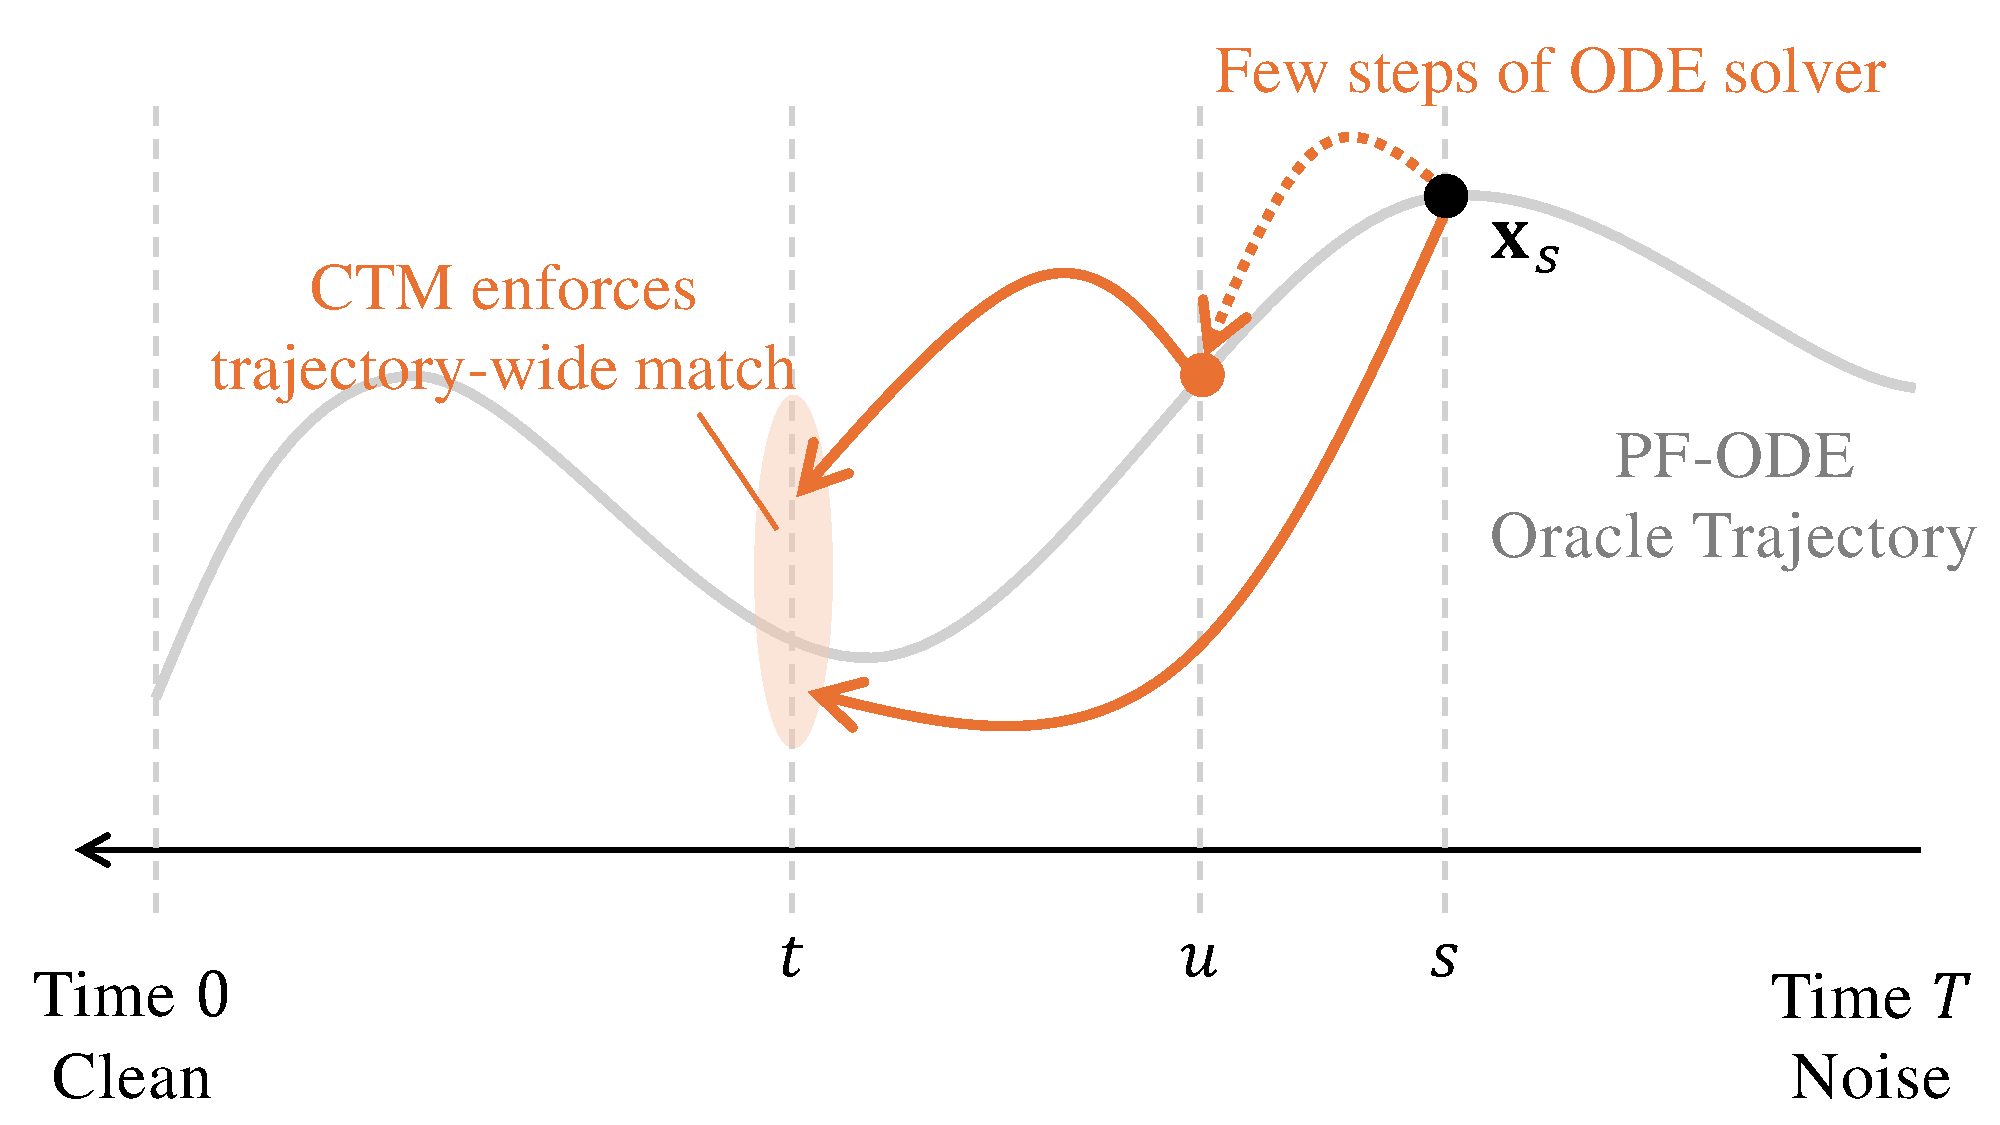
\includegraphics[width=0.9\linewidth]{Images/PartD/ctm-target.pdf}
    \caption{\textbfs{CTM 半群性质的示意图。} 对任意 $s \ge u \ge t$，CTM 强制
    $\rmG_{\btheta}(\rvx_s, s,  t)
\approx
\rmG_{\btheta^-} \big(\mathtt{Solver}_{s\to u}(\rvx_s), u ,  t\big)$，
即一段短求解器段 $s \to u$ 后接一个到 $t$ 的 CTM “跳转”，匹配直接的 CTM 映射 $s\to t$。求解器可以是预训练扩散模型或 CTM 的自诱导教师。\figcredit{改编自 \citet{kim2023consistency}。}}
    \label{fig:ill_models}
\end{figure}

\subsection{CTM 中的辅助损失}\label{subsec:ctm-auxiliary}

（自）蒸馏可能表现不如教师，因为它仅对教师生成的目标进行优化，缺乏来自真实数据的直接监督。相比之下，CTM 能自然地纳入数据驱动的正则化项，例如通过在目标中增加去噪得分匹配和对抗（GAN）项~\citep{goodfellow2014generative}，以更好地学习流映射。

\paragraph{扩散损失的自然整合。}
扩散模型损失（更准确地说是条件流匹配损失；见\Cref{eq:fm-cfm}）自然地整合进 CTM，并提供一个固定的回归目标，便于流映射模型的学习。为看清这一点，注意我们有
\[
\rvv^*(\rvx_s, s)
= \frac{\rvx_s - \rvg^*(\rvx_s, s, s)}{s},
\qquad
\rvg^*(\rvx_s, s, s) \approx \rvg_{\btheta}(\rvx_s, s, s).
\]
这自然通过 $\rvg_{\btheta}$ 诱导出一个速度参数化：
\[
\rvv_{\btheta}(\rvx_s, s)
:= \frac{1}{s}\bigl(\rvx_s - \rvg_{\btheta}(\rvx_s, s, s)\bigr).
\]
使用线性高斯路径
\[
\rvx_s = \alpha_s \rvx_0 + \sigma_s \beps,
\qquad
\rvx_0 \sim p_{\mathrm{data}},
\beps \sim \mathcal N(0, \mathbf I),
\]
扩散模型损失可以写为
\begin{align}\label{eq:ctm-dsm}
\mathcal L_{\mathrm{DM}}(\btheta)
&:= 
\E_{\rvx_0, \beps, s}
\Bigl[
w(s)
\bigl\|
 \rvv_{\btheta}(\rvx_s, s) - \left(\alpha_s' \rvx_0 + \sigma_s' \beps\right)
\bigr\|_2^2
\Bigr].
\end{align}



$\mathcal L_{\mathrm{DM}}$ 在 $t$ 接近 $s$ 时通过显式监督轨迹上的小跳来提高精度。在该体系下，\Cref{eq:ctm_para_1}中的因子 $1-\tfrac{t}{s}$
接近零，可能削弱梯度并减缓
学习；$\mathcal L_{\mathrm{DM}}$ 提供更强的局部信号并稳定训练。

从概念上讲，\Cref{eq:ctm-consist-distill,eq:ctm-consist-scratch}强制
轨迹匹配（零阶），而\Cref{eq:ctm-dsm}强制
斜率匹配（一阶）。

\paragraph{(可选) GAN 损失。}
虽然一致性和扩散模型损失提供了强的回归信号，但它们可能产生
过度平滑的输出。CTM 因此可选地加入一个对抗项以
通过将生成器
分布与数据分布对齐来鼓励更锐利、更真实的样本。用一个判别器
$D_{\bm{\zeta}}$ 区分真实 $\rvx_{0}\sim p_{\mathrm{data}}$ 和
生成的 $\rvx_{\mathrm{est}}(\rvx_{s},s,t)$，目标为
\begin{align*}
&\mathcal{L}_{\mathrm{GAN}}(\bm{\theta}, \bm{\zeta}) := \\ &\mathbb{E}_{\mathbf{x}_0} \big[\log D_{\bm{\zeta}}(\mathbf{x}_0)\big] + \mathbb{E}_{s \in [0, T]} \mathbb{E}_{t \in [0, s]} \mathbb{E}_{\mathbf{x}_0} \mathbb{E}_{\mathbf{x}_s \vert \mathbf{x}_0} \big[\log (1 - D_{\bm{\zeta}}( \mathbf{x}_{\mathrm{est}}(\mathbf{x}_s, s, t)))\big], \end{align*}
其中 $D_{\bm{\zeta}}$ 被最大化，$\rmG_{\bm{\theta}}$ 被最小化。
直观上，判别器充当一个自适应的感知距离，
鼓励真实的细节。理论上，GAN 项驱动
$p_{\mathrm{data}}$ 与 $\rmG_{\bm{\theta}}$ 所诱导模型分布之间的
分布匹配（Jensen-Shannon 散度）~\citep{goodfellow2014generative}，
这可能使保真度超越教师。

\paragraph{CTM 总目标。}
总之，CTM 将（自）蒸馏、扩散和 GAN 损失统一到单一训练框架中：
\begin{mdframed}
    \begin{align*}
\mathcal{L}_{\mathrm{CTM}}(\bm{\theta},\bm{\zeta})
:=  \mathcal{L}_{\mathrm{consist}}(\bm{\theta};  \bm{\phi}^\times/\bm{\theta}^-)
+ \lambda_{\mathrm{DM}} \mathcal{L}_{\mathrm{DM}}(\bm{\theta})
+ \lambda_{\mathrm{GAN}} \mathcal{L}_{\mathrm{GAN}}(\bm{\theta},\bm{\zeta}),
\end{align*}
\end{mdframed}
其中教师或者是外部预训练模型 $\bm{\phi}^\times$，或者是
自诱导教师 $\bm{\theta}^-$。回归式分量
$\mathcal{L}_{\mathrm{consist}}$ 和 $\mathcal{L}_{\mathrm{DM}}$ 充当强
正则化项，而可选的 GAN 项在不
牺牲稳定性的前提下改善细尺度细节~\citep{kim2024pagoda}。


\subsection{使用 CTM 进行灵活采样}
CTM 学习任意 $s>t$ 的一般流映射 $\bPsi_{s\to t}$，这意味着它支持
任意时刻到任意时刻的转移。这一性质使灵活的采样策略成为可能。
例如，CTM 提出 \emph{$\gamma$ 采样}，其中超参数 $\gamma$
控制生成过程中的随机性。
此外，CTM 可以复用为扩散模型开发的标准推理技术，
例如基于 ODE 的求解器和精确似然计算。

在下文中，我们固定一个离散时间网格用于采样 $T=\tau_0 > \tau_1 > \tau_2 > \cdots > \tau_{M}=0$。

\begin{algorithm}[H]
    \centering
    \caption{CTM 的 $\gamma$-采样}\label{alg:gamma}
    \begin{algorithmic}[1]
    \Require 训练好的 CTM $\mathbf{G}_{\bm{\theta}^\times}$，$\gamma\in[0,1]$，$T=\tau_0>\tau_1 > \tau_2 > \cdots > \tau_{M}=0$。
    \State 从 $\mathbf{x}_{\tau_{0}}\sim p_{\mathrm{prior}}=\mathcal{N}(\bm{0}, T^2\rmI)$ 开始
        \For{$n=0$ 到 $M-1$}
        \State $\tilde{\tau}_{n+1}\leftarrow \sqrt{1-\gamma^{2}}\tau_{n+1}$
        \State 去噪 $\mathbf{x}_{\tilde{\tau}_{n+1}}\leftarrow \mathbf{G}_{\bm{\theta}^\times}(\mathbf{x}_{\tau_{n}},\tau_{n},\tilde{\tau}_{n+1})$
        \State 加噪 $\mathbf{x}_{\tau_{n+1}}\leftarrow\mathbf{x}_{\tilde{\tau}_{n+1}}+\gamma \tau_{n+1}\bm{\epsilon}$，其中 $\bm{\epsilon}\sim\mathcal{N}(\bm{0}, \rmI)$
        \EndFor
        \Ensure  $\mathbf{x}_{\tau_{M}}$
    \end{algorithmic}
\end{algorithm}

\paragraph{$\gamma$-采样方法论。}
CTM 的 $\gamma$-采样引入了一个统一的采样器家族，它自然地产生于学习一般流映射模型。
它涵盖了先前的方法，例如 CM 的多步采样（见\Cref{alg:cm_sampling}）
以及时间步进式采样，后者在概念上类似于 ODE 求解器。
参数 $\gamma$ 直接控制生成过程中语义变化的程度，
使 $\gamma$ 采样成为针对多样下游应用的灵活且任务感知的策略。





\begin{figure}[t]
    \centering
    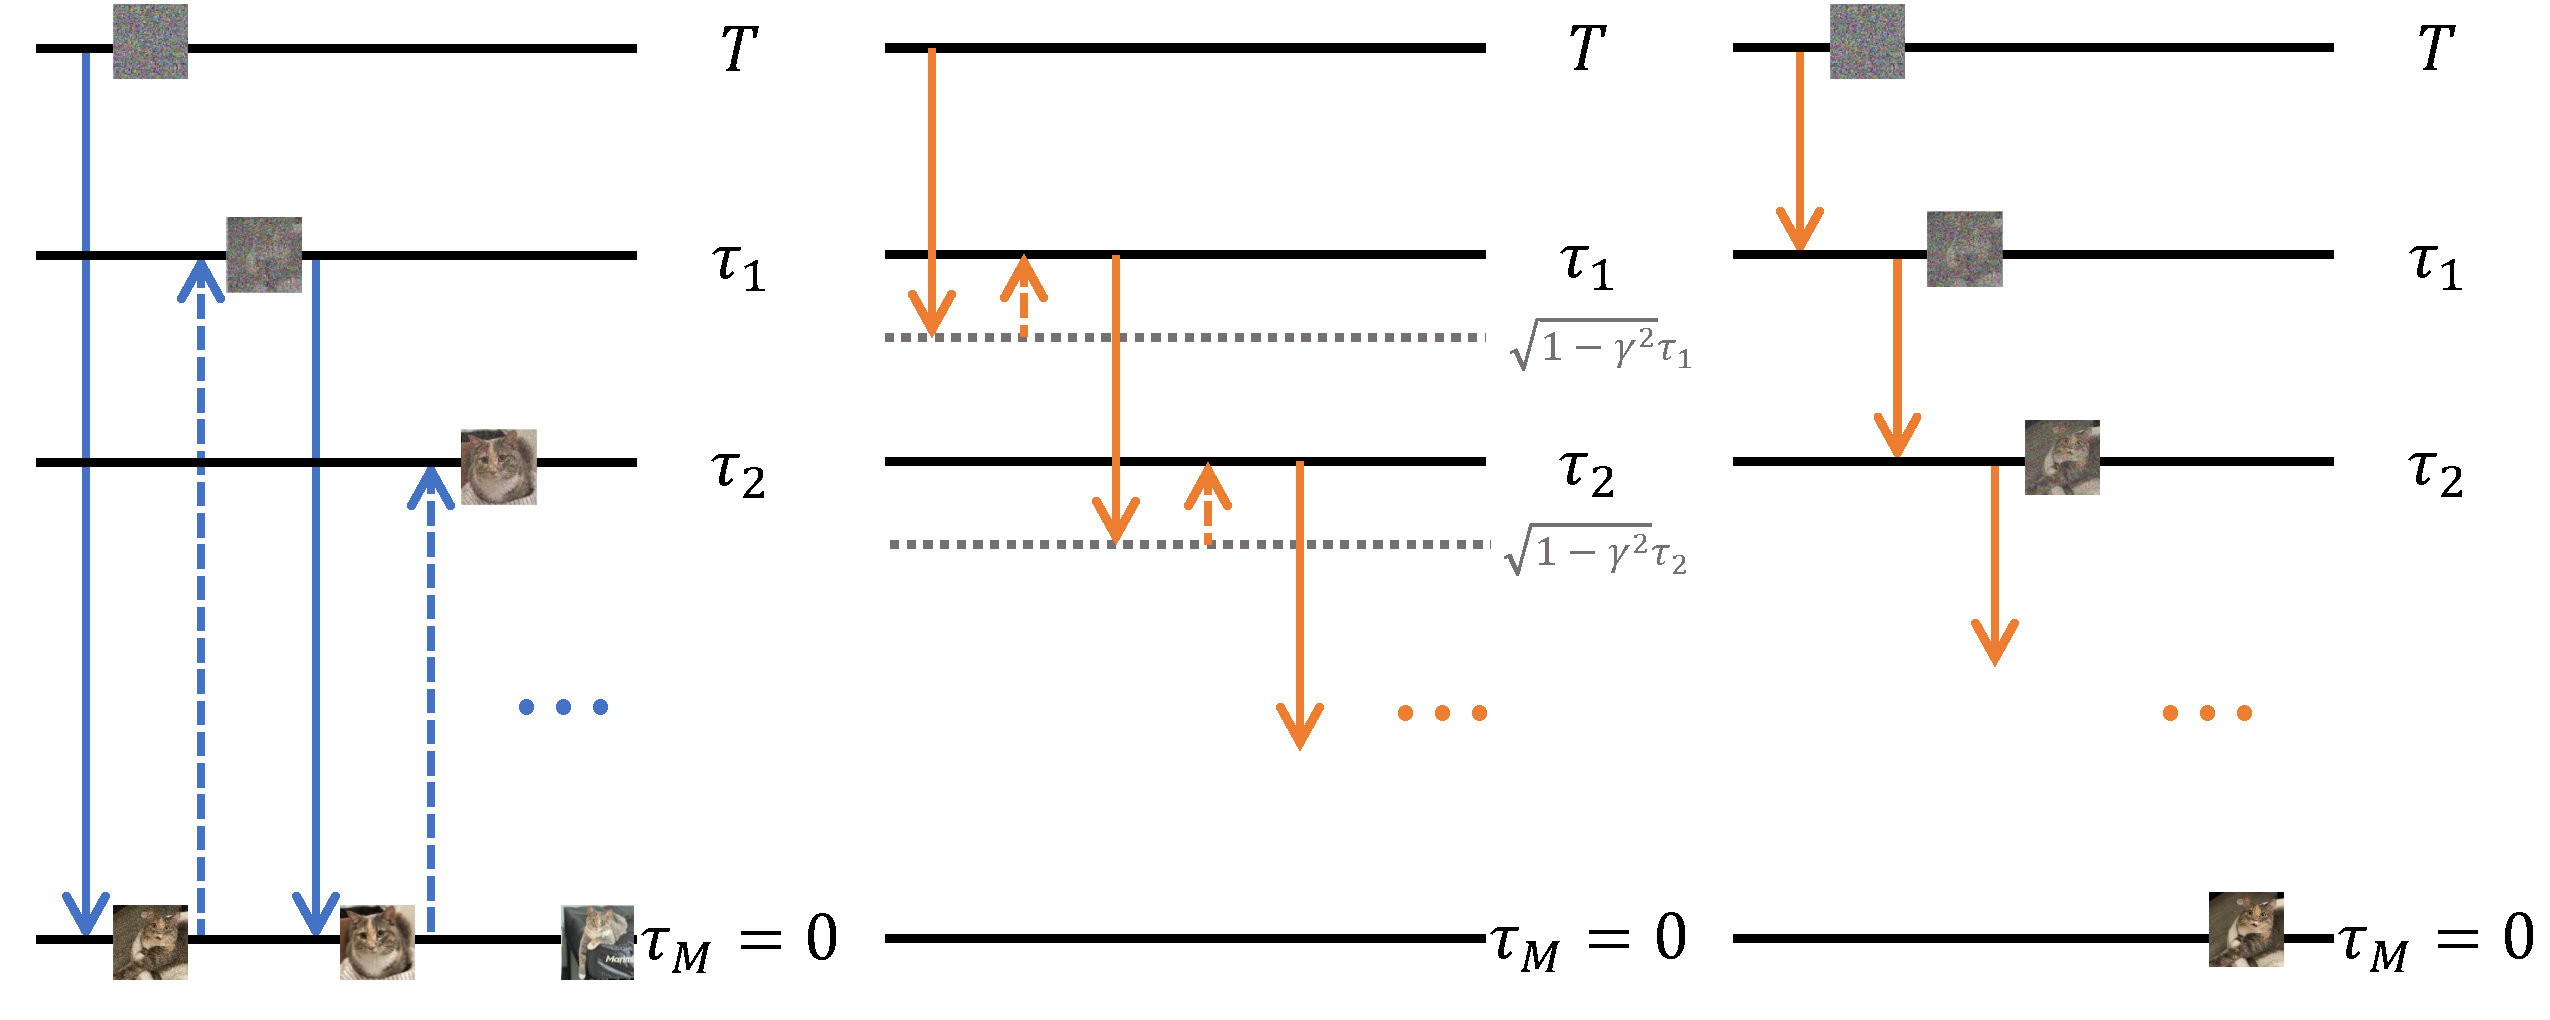
\includegraphics[width=\linewidth]{Images/PartD/ctm_gamma.pdf}
    \caption{\textbfs{不同 $\gamma$ 值下 $\gamma$-采样的示意图。} 该过程在网络求值去噪与反向加噪之间交替，   $(\tau_{n}\xrightarrow{\text{去噪}} \sqrt{1-\gamma^{2}}\tau_{n+1}\xrightarrow{\text{加噪}} \tau_{n+1})_{n=0}^{M-1}$。
最左边的面板展示了 $\gamma=1$，对应完全随机的情形。
最右边的面板展示了 $\gamma=0$，对应完全确定的情形。
中间的面板描绘了中间值 $\gamma\in(0,1)$，在两个极端之间插值。
\figcredit{改编自 \citet{kim2023consistency}。}}
    \label{fig:gamma_sampling}
\end{figure}


\begin{itemize}
\item \Cref{fig:gamma_sampling}-（左）：当 $\gamma=1$ 时，它恰好与 CM 中引入的多步采样（即特殊流映射 $\bPsi_{s\to 0}$）重合，是完全随机的，并在步数变化时产生语义变化。

\item \Cref{fig:gamma_sampling}-（右）：当 $\gamma=0$ 时，它退化为完全确定时间步进，估计 PF-ODE 的解轨迹。$\gamma=0$ 的 $\gamma$ 采样与传统基于时间步进 ODE 的采样之间的一个关键区别是，CTM 避免了数值求解器的离散化误差。

\item \Cref{fig:gamma_sampling}-（中）：当 $0 < \gamma < 1$ 时，$\gamma$-采样通过允许在采样过程中注入可控量的随机性，在两个极端之间插值。
\end{itemize}
我们强调，能够实现 $\gamma \in (0,1]$ 的采样器只有在模型学习一般流映射 $\bPsi_{s\to t}$ 时才可能。

\paragraph{$\gamma$-采样分析。} CTM 经验观察到，一旦步数 $M \geq 4$，CM 的多步采样质量就会下降。
为解释这一现象，CTM 分析了潜在原因：当 $\gamma \neq 0$ 时，每次神经“跳转”都会引入小的失配，而这些失配随着模型迭代地将状态映射向时刻零而累积。这种误差累积解释了为何长的多步运行可能表现不佳。我们在如下命题中将这一思想形式化。

\proppp{(非正式) 两步 $\gamma$-采样}{ctm-gamma}{
\label{th:sampling_agg_error_2_steps}
令 $\tau\in(0,T)$，$\gamma \in [0,1]$。设 $p_{\bm{\theta}^{*},2}$ 为由最优 CTM 的 $\gamma$-采样器得到的密度，遵循转移序列 $
    T\rightarrow\sqrt{1-\gamma^2}\tau\rightarrow \tau \rightarrow 0
$，从 $p_{\mathrm{prior}}$ 出发。则
 \begin{align*}
    \mathcal D_{\mathrm{TV}}\big( p_{\mathrm{data}}, p_{\bm{\theta}^{*},2} \big)         = \mathcal{O}\left(\sqrt{T-\sqrt{1-\gamma^2}\tau+ \tau}  \right).
 \end{align*}
 这里，$\mathcal{D}_{\mathrm{TV}}$ 表示分布之间的全变差距离（见\Cref{eq:f-div}）。
}{
关于采样步数为 $M$ 的一般情形，我们请读者参考 \citet{kim2023consistency} 的定理 8。 }
从上述定理得到的洞见可总结如下：
\begin{itemize}
    \item \textbfs{当} $\gamma = 1$（对应 CM 的多步采样）\textbfs{时：}该方法在每步 $n$ 进行从 $\tau_n$ 到 $0$ 的迭代长程转移。这导致量级为
    \begin{align*}
        \mathcal{O}\left(\sqrt{T + \tau_1 + \cdots + \tau_M}\right).
    \end{align*}
    的误差累积。

    \item \textbfs{当} $\gamma = 0$（对应 CTM 的确定性多步采样）\textbfs{时：}这种转移之间的时间重叠被消除。这避免了误差累积并给出更紧的界 $\mathcal{O}(\sqrt{T})$。经验上，$\gamma = 0$ 的 CTM 在采样速度和样本质量之间提供了有利的折中：增加采样步数可提升生成质量而不会引入不稳定。
\end{itemize}


\paragraph{CTM 支持扩散推理。} 由于 CTM 通过 $\rvg_{\bm{\theta}}$ 直接学习得分函数（或去噪器），
得益于其在\Cref{eq:ctm_para_1}中的参数化，它与最初为
扩散模型开发的推理技术兼容。例如，可以使用 $\rvg_{\bm{\theta}}(\cdot, s, s)$
计算精确似然
（\Cref{subsec:sde-sample}）或应用诸如 DDIM 或 DPM 的高级求解器（\Cref{ch:solvers}）
进行生成。




\newpage

\section{\texorpdfstring{一般流映射：均值流}{General Flow Map: Mean Flow}}\label{sec:MF}


正如扩散模型允许许多等价的参数化和训练目标，一般流映射 $\bPsi_{s\to t}$ 也可以通过多种合理的方式来学习。
在本节中，我们介绍\emph{均值流}（MF）~\citep{geng2025mean}，它是通用流映射族 $\bPsi_{s\to t}$ 的一个较晚的代表，展示了一种不同但有原则的视角，说明这类映射如何被有效地学习。



\subsection{均值流的建模与训练}

与建立在 EDM 框架上的 CM 和 CTM 不同，MF 基于
流匹配公式（对 $t\in[0,1]$，$\alpha_t = 1-t$，$\sigma_t  = t$）。
MF 不是直接对流映射进行参数化，而是学习区间 $[t,s]$（$t<s$）上的\emph{平均漂移}：
\[
\rvh_{\btheta}(\rvx_s, s, t)  \approx
\rvh^*(\rvx_s, s, t) := \frac{1}{t-s}\int_s^t \rvv^*(\rvx_u,u) \diff u.
\]
相应的 oracle 损失为
\begin{align}\label{eq:mf-oracle}
\mathbb{E}_{t<s} \mathbb{E}_{\rvx_s\sim p_s}\Big[w(s)
\|\rvh_{\btheta}(\rvx_s,s,t) - \rvh^*(\rvx_s,s,t)\|_2^2\Big].
\end{align}
特别地，当 $s \to t$ 时，损失函数退化为流匹配损失：
\begin{align}\label{eq:mf-to-fm}
    \mathbb{E}_{t} \mathbb{E}_{\rvx_t\sim p_t}\Big[w(t)
\|\rvh_{\btheta}(\rvx_t,t,t) - \rvv^*(\rvx_t,t)\|_2^2\Big],
\end{align}
学习的是瞬时速度。
我们在后文\Cref{subsec:equivalence-ctm-mf}中将看到，MF 与
\Cref{eq:general-cm-loss:rep}中的一般目标保持一致，
但从一个不同（然而等价）的视角来处理它。
由于 oracle 回归目标 $\rvh^*(\rvx_s,s,t)$ 一般没有闭式，MF 通过对恒等式
\[
(t-s)\,\rvh^*(\rvx_s,s,t) = \int_s^t \rvv^*(\rvx_u,u)\,\diff u
\]
关于 $s$ 求导所得的恒等式来构造一个代理。这给出\emph{MF 恒等式}：
\begin{align}\label{eq:mf-identity}
\begin{aligned}
    \rvh^*(\rvx_s,s,t)
&= \rvv^*(\rvx_s,s) - (s-t) \tfrac{\diff}{\diff s}\rvh^*(\rvx_s,s,t) \\
&= \rvv^*(\rvx_s,s) - (s-t)\Big[(\partial_{\rvx}\rvh^*)(\rvx_s,s,t) \rvv^*(\rvx_s,s) 
+ \partial_s \rvh^*(\rvx_s,s,t)\Big],
\end{aligned}
\end{align}
其中第二行应用链式法则以及
\[
\frac{\diff}{\diff s}\rvx_s = \rvv^*(\rvx_s,s).
\]

受此恒等式启发，MF 用一个停梯度代理替代不可达的 oracle，得到实用的训练目标
\begin{mdframed}
\begin{align}\label{eq:mf-practice}
    \mathcal{L}_{\mathrm{MF}}(\btheta)
:= \mathbb{E}_{t<s} \mathbb{E}_{\rvx_s\sim p_s}\Big[w(s)\,
\|\rvh_{\btheta}(\rvx_s,s,t) - \rvh_{\btheta^-}^{\mathrm{tgt}}(\rvx_s,s,t)\|_2^2\Big],
\end{align}
\end{mdframed}
其中回归目标定义为
\begin{align*}
    \rvh_{\btheta^-}^{\mathrm{tgt}}&(\rvx_s,s,t)
:= \\ &\rvv^*(\rvx_s,s) - (s-t)\Big[\underbrace{(\partial_{\rvx}\rvh_{\btheta^-})(\rvx_s,s,t) \rvv^*(\rvx_s,s)
+ \partial_s \rvh_{\btheta^-}(\rvx_s,s,t)}_{\mathrm{JVP}}\Big].
\end{align*}

实践中，oracle 速度 $\rvv^*$ 不能以闭式计算，
必须被近似。有两种常见策略：依赖
预训练扩散模型（\emph{蒸馏}）或从数据中构造直接
估计器（\emph{从零开始训练}）。无论作何选择，最终都需要计算目标网络
$\rvh_{\btheta^-}$ 的一个\emph{雅可比-向量积}（JVP）：
\[
\left[\partial_\rvx \rvh_{\btheta^-}, \partial_s \rvh_{\btheta^-}, \partial_t \rvh_{\btheta^-}\right]^\top \cdot \left[\rvv^*, 1, 0\right]
\]


\paragraph{蒸馏。}
使用具有流匹配骨干的预训练扩散模型，
$\rvv_{\bphi^\times} \approx \rvv^*$。

\paragraph{从零开始训练。}
使用单点条件速度 $\alpha_s'\rvx_0 + \sigma_s'\beps$，
由前向加噪 $\rvx_s=\alpha_s\rvx_0+\sigma_s\beps$ 得到，其中
$\beps\sim\mathcal N(\bm{0},\rmI)$。这给出了在配对 $(\rvx_0,\beps)$ 处求值时层级 $s$ 瞬时漂移的无偏单样本估计。

% We emphasize that MF’s strength lies in its strong performance in the training-from-scratch setting. It requires no pre-trained model for initialization or guidance during training, and it does not rely on additional regularizers (such as a GAN loss). In this sense, MF serves as a fully standalone generative model.

\subsection{均值流的采样}
一旦均值流 $\rvh_{\btheta^\times}$ 训练完成，它自然地恢复出流映射的一个代理。对任意起点 $\rvx_s$，从 $s$ 到 $t$ 的映射（近似）为
\[
\bPsi_{s\to t}(\rvx_s) = \rvx_s + (t-s)\,\rvh^*(\rvx_s,s,t)
  \approx   \rvx_s + (t-s)\,\rvh_{\btheta^\times}(\rvx_s,s,t).
\]

这使得单步和多步采样都成为可能。例如，抽取
$\rvx_T\sim p_{\mathrm{prior}}$，干净样本的单步生成为
\[
\rvx_0  \leftarrow  \rvx_T + T\,\rvh_{\btheta^\times}(\rvx_T,T,0).
\]

或者，可以通过准备一个时间网格并按序施加映射
来进行多步生成，采用与
CTM 相同的时间步进方式。由于 MF 学习的是一般流映射，它也支持
CTM 中的 $\gamma$-采样，其中可控超参数 $\gamma$ 向采样过程注入随机性。



\subsection{CTM 与 MF 之间的关系}\label{subsec:equivalence-ctm-mf}
乍看之下，CTM 与 MF 似乎并不相关。
事实上，两者都只是同一 oracle 流映射 $\bPsi_{s\to t}$ 的不同参数化，它们的训练损失（CTM 的一致性损失与\Cref{eq:mf-oracle}）仅在时间加权上有所不同~\citep{hu2025cmt}。

\paragraph{参数化之间的关系。}
两种方法都在同一一般框架下运作，但以不同的方式表示所学函数。
流映射可以等价写为
\begin{align*}
\bPsi_{s\to t}(\rvx_s)
& = \rvx_s + \int_s^t \rvv^*(\rvx_u, u)\diff u \\
&= \frac{t}{s}\rvx_s
   + \frac{s-t}{s}\underbrace{\Bigg[\rvx_s + \frac{s}{s-t}\int_s^t \rvv^*(\rvx_u,u)\,\diff u\Bigg]}_{\approx\,\rvg_\btheta} \\
&= \rvx_s + (t-s)\underbrace{\Bigg[\frac{1}{t-s}\int_s^t \rvv^*(\rvx_u,u)\,\diff u\Bigg]}_{\approx\,\rvh_\btheta}.
\end{align*}
这里，第一个是流映射的定义，第二个形式通过 $\rvg_\btheta$ 突出 CTM 参数化（见\Cref{eq:ctm-g-oracle,eq:ctm_para_1}），最后一个通过 $\rvh_\btheta$ 突出 MF 参数化。


\paragraph{训练损失之间的关系。} 给定上述用 CTM 参数化对 oracle 流映射 $\bPsi_{s\to t}$ 的重新解释
\[
\rvg_\btheta(\rvx_s,s,t) \approx \rvg^*(\rvx_s,s,t):=\rvx_s + \frac{s}{s-t}\int_s^t \rvv^*(\rvx_u,u) \diff u
\]
 和 MF 参数化
\[
\rvh_\btheta(\rvx_s,s,t) \approx \rvh^*(\rvx_s,s,t):=\frac{1}{t-s}\int_s^t \rvv^*(\rvx_u,u) \diff u,
\]
我们现在说明 CTM 和 MF 的训练损失实际上是等价的。


考虑关系
\[
\rvg_\btheta(\rvx_s,s,t) := \rvx_s - s \rvh_\btheta(\rvx_s,s,t),
\]
并以 $d(\rvx,\rvy):=\|\rvx-\rvy\|^2$ 为例。代入\Cref{eq:general-cm-loss:rep}并将 $\rmG_\btheta$ 视为 CTM 的流映射参数化（\Cref{eq:ctm_para_1}）得到
\begin{align} &~d\big(\rmG_\btheta(\rvx_s,s,t), \bPsi_{s\to t}(\rvx_s)\big) \notag \\ = &~\norm{\rmG_\btheta(\rvx_s,s,t) - \bPsi_{s\to t}(\rvx_s)}^2 \notag \\ = &~\norm{\left(\frac{t}{s}\rvx_s + \frac{s-t}{s} \rvg_\btheta(\rvx_s,s,t)\right)-\left(\frac{t}{s}\rvx_s + \frac{s-t}{s}\Big[\rvx_s + \frac{s}{s-t}\int_s^t \rvv^*(\rvx_u,u) \diff u\Big]\right)}^2 \notag \\ = &~\left(\frac{s-t}{s}\right)^2\norm{\rvg_\btheta(\rvx_s,s,t)-\left(\rvx_s + \frac{s}{s-t}\int_s^t \rvv^*(\rvx_u,u) \diff u\right)}^2 \label{eq:g-para} \\ = &~\left(\frac{s-t}{s}\right)^2\norm{\left(\rvx_s - s \rvh_\btheta(\rvx_s,s,t)\right)-\left(\rvx_s + \frac{s}{s-t}\int_s^t \rvv^*(\rvx_u,u) \diff u\right)}^2 \notag \\ = &~\left(\frac{s-t}{s}\right)^2\norm{\left(\rvx_s - s \rvh_\btheta(\rvx_s,s,t)\right)-\left(\rvx_s + \frac{s}{s-t}\int_s^t \rvv^*(\rvx_u,u) \diff u\right)}^2 \notag \\ = &~\left(s-t\right)^2\norm{ \rvh_\btheta(\rvx_s,s,t)- \left(\frac{1}{t-s}\int_s^t \rvv^*(\rvx_u,u)\diff u \right)}^2 \label{eq:h-para} \end{align}
 因此，
\begin{align*}
\frac{1}{s^2} \Bigg\|\rvg_\btheta(\rvx_s,s,t)-\rvg^*(\rvx_s,s,t) \Bigg\|^2 = \Bigg\|\rvh_\btheta(\rvx_s,s,t)-\rvh^*(\rvx_s,s,t) \Bigg\|^2.
\end{align*}
撇开用于学习流映射的具体算法不谈，CTM 和 MF 的损失具有相同的数学形式，仅相差一个加权函数。此外，在两种情形中令 $t=0$ 都恢复 CM 的设定（$\bPsi_{s\to 0}$），其中
每个状态直接映射到干净数据。

\paragraph{实践中的辅助损失。}
在 CTM 中，训练是用\Cref{eq:ctm-consist-scratch}中的一致性损失与\Cref{eq:ctm-dsm}中其自定义的扩散模型损失联合进行的。MF 采用了类似的策略。如\Cref{eq:mf-to-fm}所示，当 $s \to t$ 时，MF 损失退化为标准流匹配目标。实践中，MF 控制 $s \neq t$ 对与 $s = t$ 对之间的比例；因此，整体优化变成\Cref{eq:mf-practice}中 MF 目标与\Cref{eq:mf-to-fm}中流匹配目标的混合。

两种参数化都能够实现从扩散模型训练（以固定回归目标学习瞬时速度）到流映射学习（采用停梯度伪回归目标）的平滑过渡。


\paragraph{CTM 和 MF 参数化都支持灵活推理。}
CTM（$\rmG_\btheta(\rvx_s,s,t)$）和 MF（$\rvh_\btheta(\rvx_s,s,t)$）都旨在近似底层流映射 $\bPsi_{s\to t}$：
\[
\rmG_\btheta(\rvx_s,s,t)\approx\bPsi_{s\to t},\quad  \text{且}
\quad
\rvx_s+(t-s)\rvh_\btheta(\rvx_s,s,t)\approx\bPsi_{s\to t}.
\]
由于两个模型都学习任意两个时间步之间的显式映射，它们自然支持 CTM 的 $\gamma$-采样，并与最初为扩散模型开发的推理技术兼容，例如引导（\Cref{ch:guidance}）、精确似然计算（\Cref{eq:score-sde-likelihood}）以及使用高阶求解器的加速采样（\Cref{ch:solvers}）。
这种兼容性源于它们的参数化在无穷小极限 $t\to s$ 下恢复瞬时扩散漂移：
\[
\rvg^*(\rvx_s,s,s)=\rvx_s-\rvv^*(\rvx_s,s),
\quad  \text{且}
\quad
\rvh^*(\rvx_s,s,s)=\rvv^*(\rvx_s,s).
\]
特殊化流映射公式 $\bPsi_{s\to0}$（如 CM 系列）不具备这一性质。因此，CTM 和 MF 都可视为灵活、一般的流映射公式，将基于扩散的推理推广到直接的时间到时间映射。




\paragraph{结论。}
% This equivalence between CTM and MF is similar to the situation in diffusion models (\Cref{sec:equivalent-parametrizations}), where different parameterizations ultimately describe the same underlying oracle target. In principle, these formulations are mathematically identical. In practice, however, their behavior can differ because of factors such as loss weighting, network design, or optimization dynamics, which may cause one approach to perform better than another under specific conditions.


CTM 与 MF 之间的关系类似于扩散模型中的情形（\Cref{sec:equivalent-parametrizations}），不同的参数化最终描述的是同一底层 oracle 目标。就学习对象而言，这些公式在数学上是等价的；在损失目标层面，它们可视为等价。

尽管 CTM 和 MF 存在这种关联，它们在学习目标的方式上，无论在概念上还是算法上都有所不同。CTM 目标以“积分”形式定义，因为它直接作用于流映射。而 MF 目标以“微分”形式定义，因为它依赖于流映射的有限差分。由于积分形式的目标不可直接处理，CTM 必须在训练过程中求解一个 ODE。相比之下，MF 利用 MF 恒等式（见\Cref{eq:mf-identity}）构造一个可处理的微分形式目标。这种关系类似于基于能量与基于得分方法之间的关系：前者学习概率密度本身（积分形式），后者匹配该密度的梯度（微分形式）。实践中，由于损失加权、网络架构和优化动力学等因素，CTM 和 MF 可能表现不同，这些因素可能使一种方法在某些条件下优于另一种。

这一视角表明 CTM 和 MF 并非唯一可行的公式。流映射的其他参数化也可能实现高效、稳定的训练，潜在地带来新的独立生成模型。探索这些替代方案可能会进一步丰富扩散模型及其流映射扩展的版图，推动少步生成的边界。

\newpage

\section{结语}\label{sec:ch11_cr}

本章为我们的探索画上了完整的闭环：从缓慢的迭代
扩散采样器到快速的少步生成器（从零开始学习）。本章各方法背后的共同对象是
\Cref{eq:general-cm-loss:rep}中引入的 oracle 流映射：
\[
\bPsi_{s\to t}(\rvx_s)
=
\rvx_s+\int_s^t \rvv^*(\rvx_\tau,\tau)\,\diff \tau.
\]
学习该映射用一次或少数几次学习到的跳转
取代了大量小的数值更新。

至此，跳出单个算法来看是有益的。
知识蒸馏（\Cref{sec:distillation-prologue}）、渐进式蒸馏（\Cref{sec:PD}）、CM（\Cref{sec:discrete-cm}）、CTM
（\Cref{sec:CTM}）和 MF（\Cref{sec:MF}）通过不同的
训练构造引入，但它们都显式或隐式地利用了相同的
ODE 解映射结构。\citet{boffi2024flow} 的流映射框架
为精确刻画这一共同结构提供了一种后来的系统性语言\footnote{我们在本部分的表述和插图也受到
\citet{dieleman2026flowmaps} 清晰论述的启发。}。在这一视角下，同一 oracle 流映射可通过三种
数学上等价的视角来解读：\emph{半群视角}、
\emph{拉格朗日视角}和\emph{欧拉视角}。这些视角提供了一种
有原则且经典的方式来描述 ODE 流下的粒子输运，
在此作为上述方法的一种组织透镜，
同时保留每种方法独特的算法贡献。

\paragraph{半群视角：拆分行程。}
如\Cref{eq:semi-group}中所引入，有限步恒等式为
\[
\bPsi_{u\to t}\big(\bPsi_{s\to u}(\rvx_s)\big)
=
\bPsi_{s\to t}(\rvx_s).
\]
如\Cref{fig:semigroup}所示，其直觉与沿固定路线行进相同：从 $s$ 到
$u$ 再从 $u$ 到 $t$，与直接从
$s$ 到 $t$ 到达同一点。在此视角下，KD 是退化的全程跳转情形 $\bPsi_{T\to0}$，PD
将两个相邻教师步压缩为一个学生步，CM 学习
特殊的任意时刻到干净样本的映射 $\bPsi_{s\to0}$，而 CTM 将同样的
复合原则推广到一般映射 $\bPsi_{s\to t}$。

\begin{figure}[t]
    \centering

    \begin{subfigure}[t]{0.485\textwidth}
        \centering
        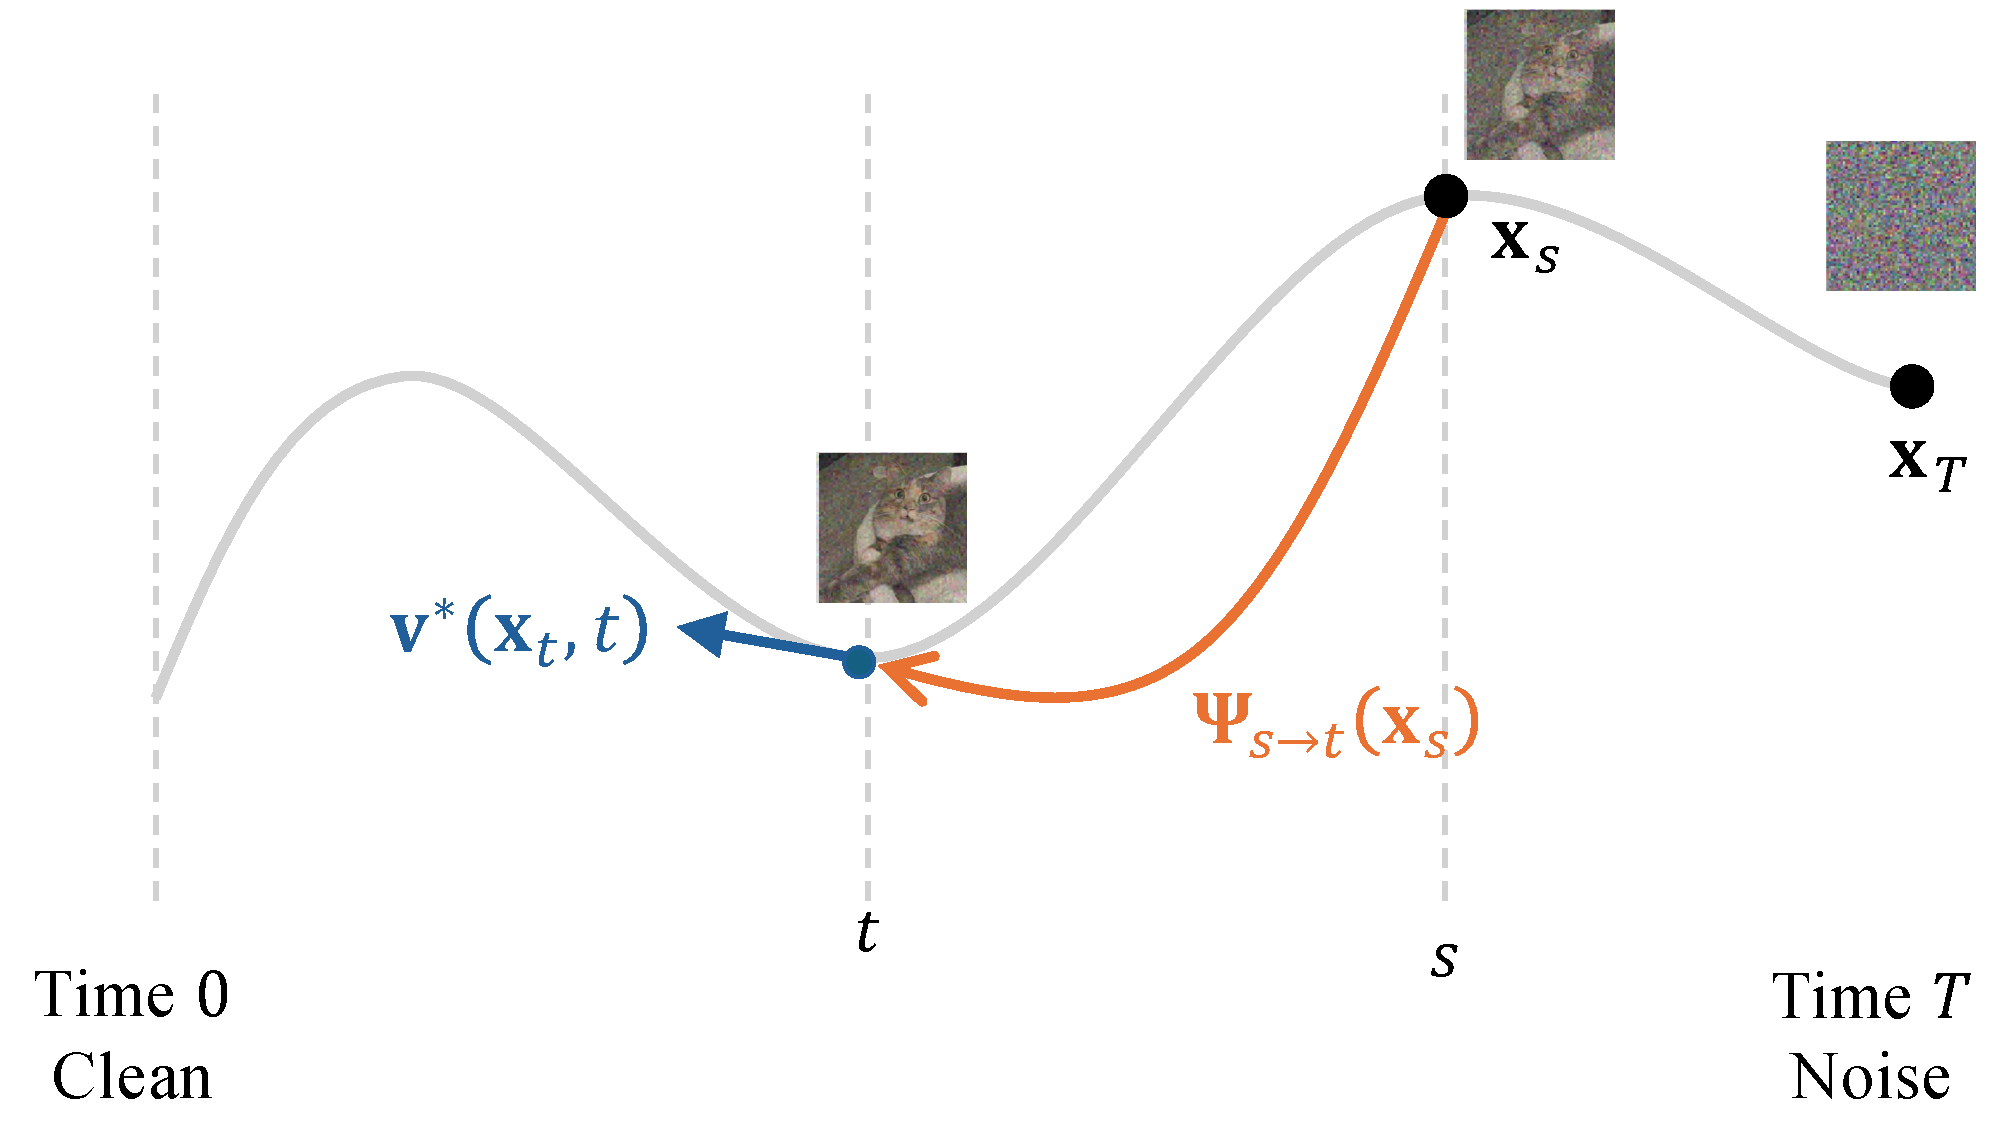
\includegraphics[width=\linewidth]{Images/PartD/lagrangian-1.pdf}
        \caption{基准目标时刻 $t$。}
        \label{fig:lagrangian-base}
    \end{subfigure}
    \hfill
    \begin{subfigure}[t]{0.485\textwidth}
        \centering
        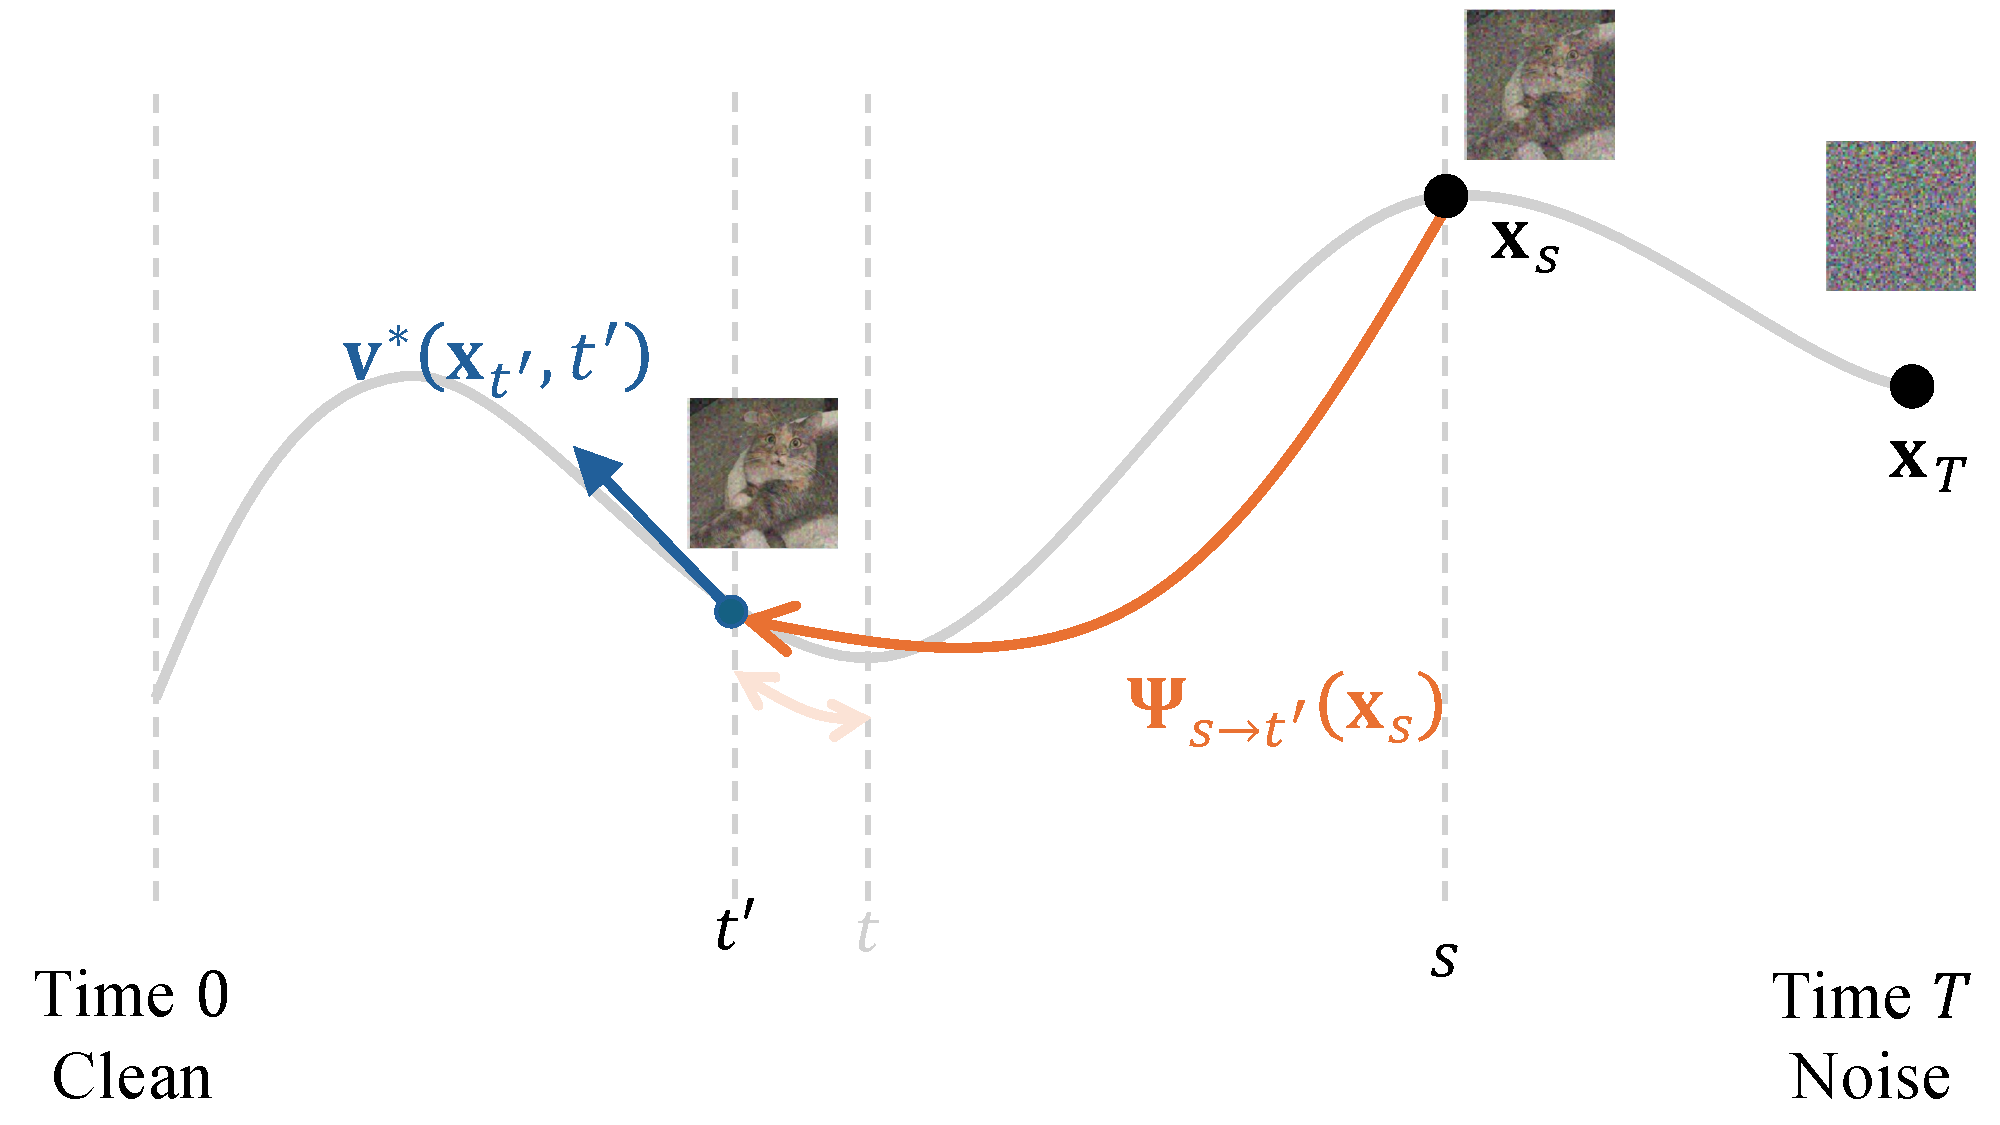
\includegraphics[width=\linewidth]{Images/PartD/lagrangian-2.pdf}
        \caption{移动后的目标时刻 $t'$。}
        \label{fig:lagrangian-moved}
    \end{subfigure}

    \caption{\textbfs{流映射的拉格朗日一致性。}
    源 $(\rvx_s,s)$ 固定，目标时刻从 $t$ 移动到
    $t'$。流映射的输出沿同一 PF-ODE 轨迹移动，其
    无穷小变化等于 ODE 速度：
    $\partial_t \bPsi_{s\to t}(\rvx_s)
    = \rvv^*(\bPsi_{s\to t}(\rvx_s),t)$。}
    \figcredit{改编自 \citet{dieleman2026flowmaps}。}
    \label{fig:lagrangian-consistency}
\end{figure}

\paragraph{拉格朗日视角：移动目的地。}
固定源 $(\rvx_s,s)$ 并移动目标时刻 $t$。预测的
终点应沿同一轨迹滑动：
\[
\partial_t \bPsi_{s\to t}(\rvx_s)
=
\rvv^*(\bPsi_{s\to t}(\rvx_s),t).
\]
“拉格朗日”这一名称源于经典的粒子视角：当目的地时刻变化时，我们追踪
轨迹上的一个移动点。在无穷小意义上，
终点以该终点处的局部 ODE 速度移动。

\paragraph{欧拉视角：移动源。}
固定目标时刻 $t$，并沿同一轨迹滑动源点。
时刻 $t$ 处的目的地保持不变：
\[
\frac{\diff}{\diff s}\bPsi_{s\to t}(\rvx_s)=0.
\]
由于 $\frac{\diff}{\diff s}\rvx_s=\rvv^*(\rvx_s,s)$，链式法则给出
\[
\partial_s\bPsi_{s\to t}(\rvx_s)
+
\big(\partial_{\rvx}\bPsi_{s\to t}\big)(\rvx_s)\rvv^*(\rvx_s,s)
=
0.
\]
“欧拉”这一名称反映了场视角：我们考察映射
如何随其源输入的变化而变化。对 CM 而言，目标是干净终点
$t=0$，且
\[
    \rvf^*(\rvx_s,s)=\bPsi_{s\to0}(\rvx_s).
\]
因此，\Cref{eq:conti-ct-motivation}是
\Cref{sec:discrete-cm,sec:conti-cm}中所研究的特殊流映射的源时刻一致性条件。



这一视角也回顾了\Cref{subsec:equivalence-ctm-mf}中
CTM 与 MF 之间的关系。两者都近似同一路径积分
\[
\bPsi_{s\to t}(\rvx_s)
=
\rvx_s+\int_s^t\rvv^*(\rvx_\tau,\tau)\,\diff\tau,
\]
但暴露出不同的可训练代理。CTM 通过
位移式参数化表示终点，而 MF 通过平均漂移表示同一终点
\[
\rvh^*(\rvx_s,s,t)
=
\frac{1}{t-s}\int_s^t\rvv^*(\rvx_\tau,\tau)\,\diff\tau.
\]
将
\[
\bPsi_{s\to t}(\rvx_s)=\rvx_s+(t-s)\rvh^*(\rvx_s,s,t)
\]
代入欧拉源时刻恒等式得到
\[
\rvh^*(\rvx_s,s,t)
=
\rvv^*(\rvx_s,s)
-
(s-t)
\left[
\partial_s\rvh^*(\rvx_s,s,t)
+
(\partial_{\rvx}\rvh^*)(\rvx_s,s,t)\rvv^*(\rvx_s,s)
\right].
\]
这就是基本的均值流恒等式：长区间上的平均漂移等于
源点处的瞬时漂移，再由平均漂移随源点沿同一轨迹滑动
的变化所修正。

\begin{figure}[t]
    \centering

    \begin{subfigure}[t]{0.485\textwidth}
        \centering
        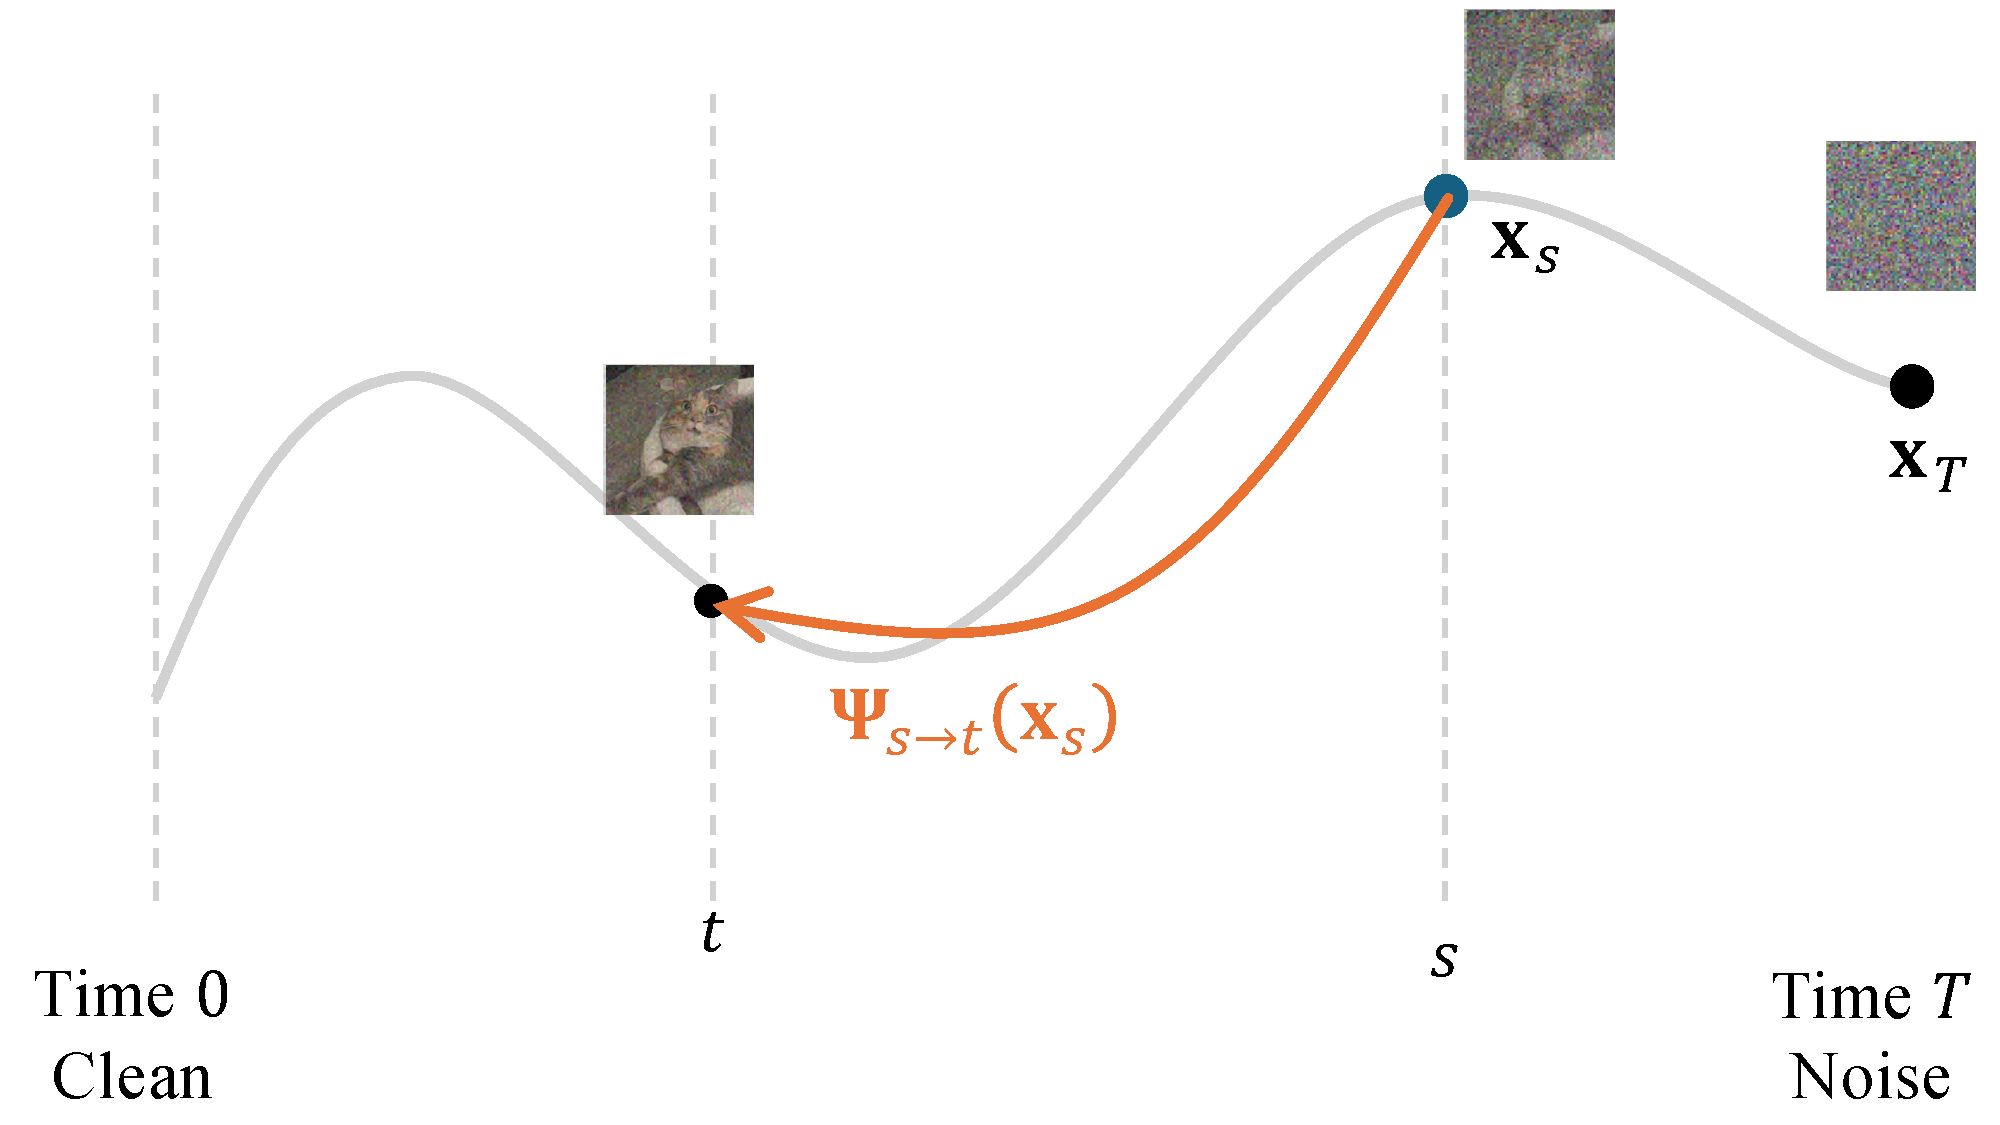
\includegraphics[width=\linewidth]{Images/PartD/eulerian-1.pdf}
        \caption{基准源时刻 $s$。}
        \label{fig:eulerian-base}
    \end{subfigure}
    \hfill
    \begin{subfigure}[t]{0.485\textwidth}
        \centering
        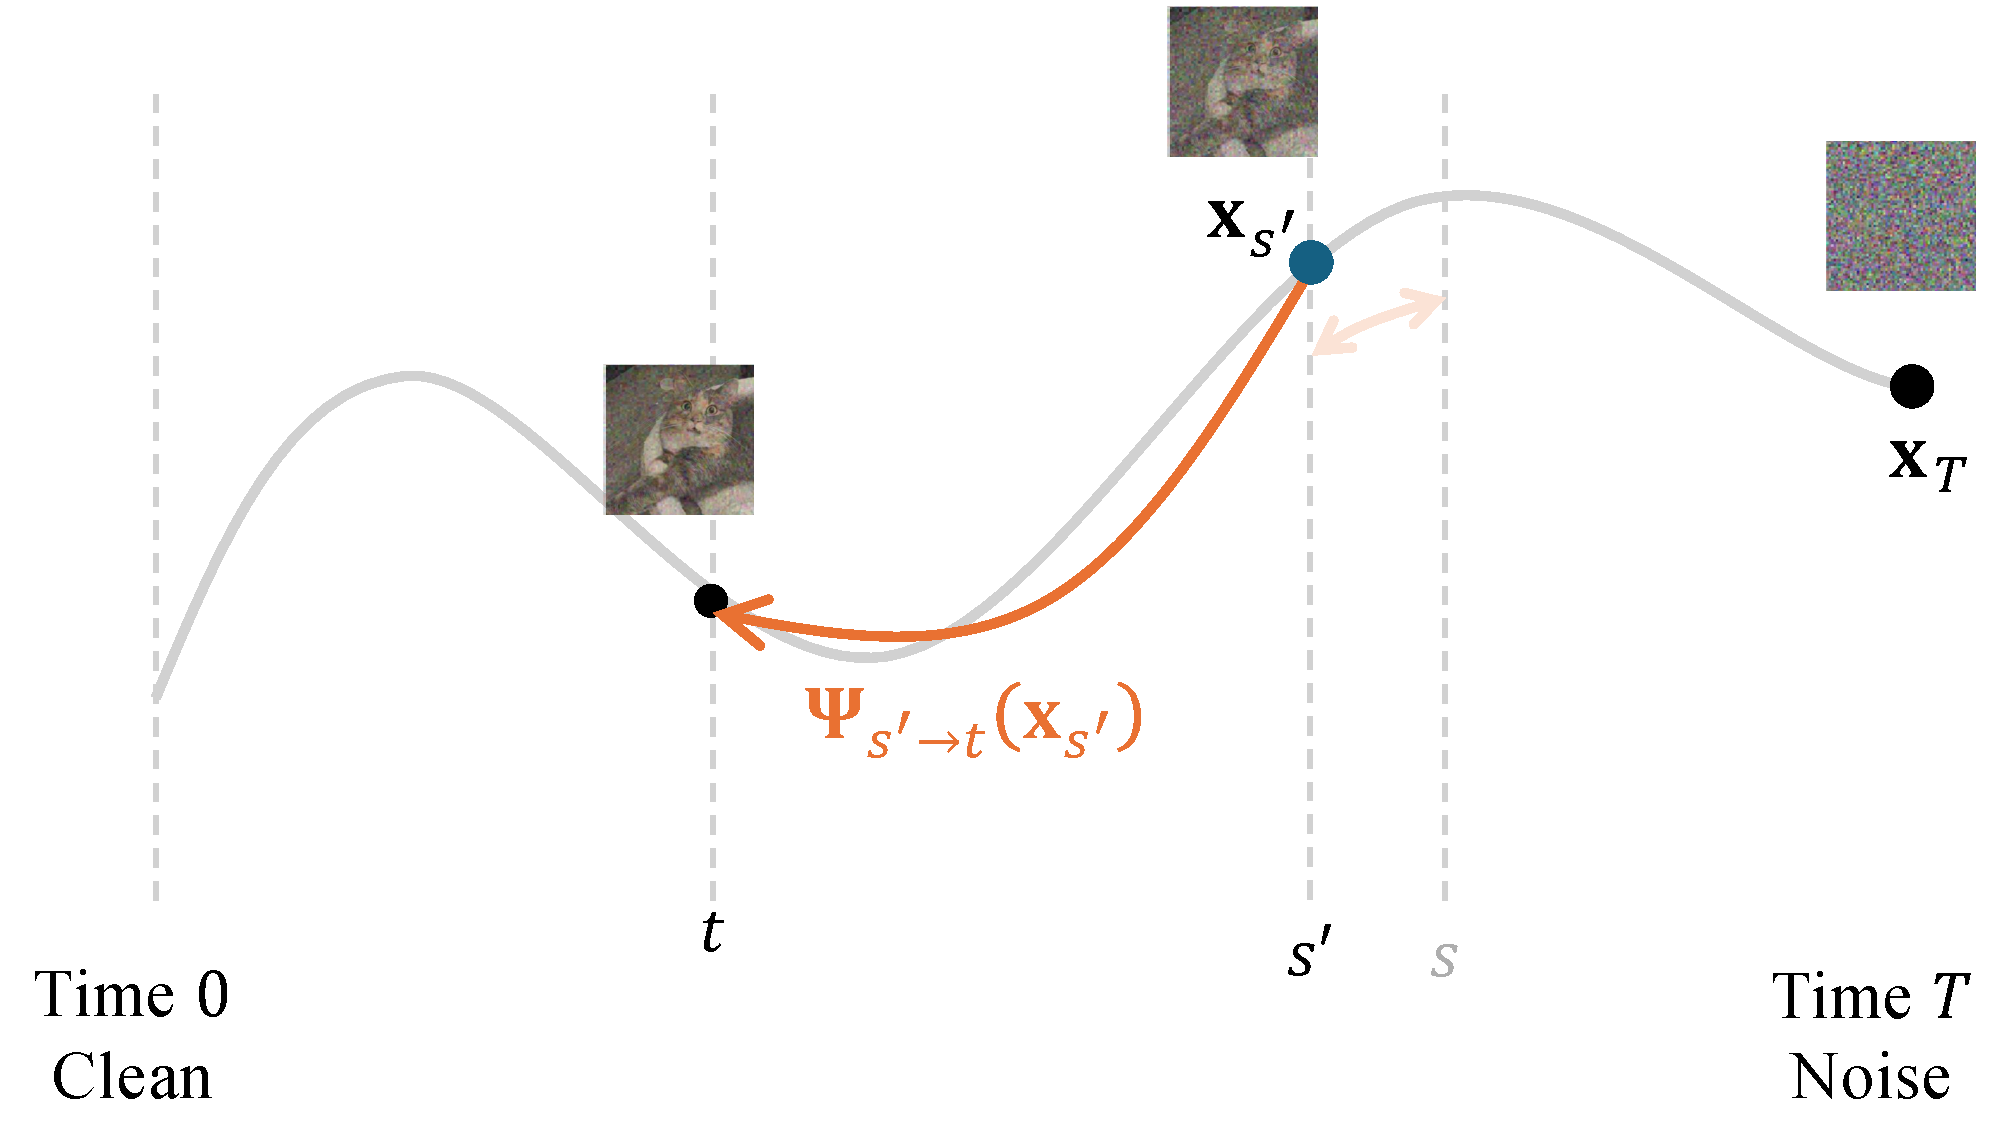
\includegraphics[width=\linewidth]{Images/PartD/eulerian-2.pdf}
        \caption{移动后的源时刻 $s'$。}
        \label{fig:eulerian-moved}
    \end{subfigure}

    \caption{\textbfs{流映射的欧拉一致性。}
    目标时刻 $t$ 固定，源时刻从 $s$ 移动到
    $s'$。由于源点位于同一 PF-ODE 轨迹上，流映射的
    输出应保持不变：
    $\bPsi_{s\to t}(\rvx_s)=\bPsi_{s'\to t}(\rvx_{s'})$。
    在无穷小意义上，这给出
    $\frac{\diff}{\diff s}\bPsi_{s\to t}(\rvx_s)=0$，或等价地
    $\partial_s\bPsi_{s\to t}(\rvx_s)
    +(\partial_{\rvx}\bPsi_{s\to t})(\rvx_s)\rvv^*(\rvx_s,s)=0$。}
        \figcredit{改编自 \citet{dieleman2026flowmaps}。}
    \label{fig:eulerian-consistency}
\end{figure}
\paragraph{三种视角的等价性。}
对于精确的 oracle 映射，半群、拉格朗日和欧拉视角是
同一 ODE 流映射的三种等价刻画~\citep{boffi2024flow}。
关键原理是 ODE 解轨迹的存在性与唯一性：
一旦状态-时刻对 $(\rvx_s,s)$ 固定，穿过它的轨迹就被
确定。

半群恒等式给出该原理的有限区间形式：
\[
    \bPsi_{u\to t}\big(\bPsi_{s\to u}(\rvx_s)\big)
    =
    \bPsi_{s\to t}(\rvx_s),
    \qquad
    \bPsi_{s\to s}=\rmI .
\]
两种微分视角通过收缩两个区间之一得到。

首先，收缩目标侧区间。对 $\Delta t>0$，
\[
    \bPsi_{t\to t-\Delta t}
    \big(\bPsi_{s\to t}(\rvx_s)\big)
    =
    \bPsi_{s\to t-\Delta t}(\rvx_s).
\]
令 $\rvx_t:=\bPsi_{s\to t}(\rvx_s)$。对短
流的一阶展开给出
\[
    \bPsi_{t\to t-\Delta t}(\rvx_t)
    =
    \rvx_t-\Delta t\,\rvv^*(\rvx_t,t)
    +\mathcal{O}\big((\Delta t)^2\big).
\]
因此，
\[
    \frac{
    \bPsi_{s\to t-\Delta t}(\rvx_s)
    -
    \bPsi_{s\to t}(\rvx_s)}
    {-\Delta t}
    =
    \rvv^*(\rvx_t,t)
    +\mathcal{O}(\Delta t).
\]
取 $\Delta t\to0$ 得到拉格朗日恒等式
\[
    \partial_t\bPsi_{s\to t}(\rvx_s)
    =
    \rvv^*\big(\bPsi_{s\to t}(\rvx_s),t\big).
\]
因此，当源 $(\rvx_s,s)$ 固定而目标时刻移动时，
预测终点以该终点处的 ODE 速度移动。

其次，收缩源侧区间。对 $\Delta s>0$，
\[
    \rvx_{s-\Delta s}
    :=
    \bPsi_{s\to s-\Delta s}(\rvx_s)
    =
    \rvx_s-\Delta s\,\rvv^*(\rvx_s,s)
    +\mathcal{O}\big((\Delta s)^2\big).
\]
半群恒等式给出
\[
    \bPsi_{s-\Delta s\to t}(\rvx_{s-\Delta s})
    =
    \bPsi_{s\to t}(\rvx_s).
\]
对左侧在源状态和源时刻上同时展开给出
\[
    \bPsi_{s-\Delta s\to t}(\rvx_{s-\Delta s})
    =
    \bPsi_{s\to t}(\rvx_s)
    -
    \Delta s\,
    \big(\partial_{\rvx}\bPsi_{s\to t}\big)(\rvx_s)\rvv^*(\rvx_s,s)
    -
    \Delta s\,
    \partial_s\bPsi_{s\to t}(\rvx_s)
    +
    \mathcal{O}\big((\Delta s)^2\big).
\]
与半群恒等式比较并除以 $-\Delta s$ 得到
\[
    \partial_s\bPsi_{s\to t}(\rvx_s)
    +
    \big(\partial_{\rvx}\bPsi_{s\to t}\big)(\rvx_s)\rvv^*(\rvx_s,s)
    =
    \mathcal{O}(\Delta s).
\]
取 $\Delta s\to0$ 得到欧拉恒等式
\[
    \partial_s\bPsi_{s\to t}(\rvx_s)
    +
    \big(\partial_{\rvx}\bPsi_{s\to t}\big)(\rvx_s)\rvv^*(\rvx_s,s)
    =
    0.
\]
这里目标时刻 $t$ 固定，而源点沿同一
轨迹移动，因此预测目的地保持不变。

反之，任一微分恒等式连同边界条件 $\bPsi_{s\to s}=\rmI$ 都恢复同一
流映射。拉格朗日恒等式从
$\bPsi_{s\to s}(\rvx_s)=\rvx_s$ 演化终点。欧拉恒等式表明
$\bPsi_{\tau\to t}(\rvx_\tau)$ 沿特征线
$\rvx_\tau=\bPsi_{s\to \tau}(\rvx_s)$ 为常数，故
\[
    \bPsi_{s\to t}(\rvx_s)
    =
    \bPsi_{t\to t}(\rvx_t)
    =
    \rvx_t.
\]
尽管这些视角在 oracle 层面等价，但一旦引入近似，它们会导致
不同的实用算法：必须
选择强制执行哪个恒等式、停梯度目标放在哪里、如何
采样时间对、以及如何参数化映射。


\paragraph{总结。}
流映射模型汇集了本书各处发展的若干原理。其概念转变是
直接学习 PF-ODE 的解映射：模型不再在采样时反复查询
局部速度场并逐步积分，而是试图将这部分积分摊销到训练中。

这一转变为单步和少步生成提供了一条有原则的路径。
当学习到的映射准确时，生成轨迹的长区间可以
仅用少量网络求值即可遍历，同时
仍然与扩散的轨迹式结构保持联系。在这个意义上，
流映射学习在迭代
扩散过程的样本质量与直接生成器的速度之间架起了一座桥梁。

代价是负担从采样转移到了学习。模型必须
近似比瞬时速度场更全局的对象，其
性能取决于参数化、时间采样、损失
加权、停梯度放置和稳定化的精心选择。
从这个角度看，从零开始学习快速生成器是基于扩散的生成式建模故事的
自然延续。它保留了使扩散模型可靠的数学
结构，同时为高效、可控、有原则的生成开启了更广阔的设计
空间。目标不再仅仅是更快地求解生成式 ODE，而是学习其
解算子本身有用的片段。



% \section{Closing Remarks}\label{sec:ch11_cr}

% This final chapter has brought our exploration full circle, culminating in a new paradigm for generative modeling: learning fast, few-step generators from scratch. Moving beyond the approaches of improving numerical solvers or distilling pre-trained models, we have focused on designing standalone training principles that are both principled and highly efficient by design.

% The core innovation presented here is the direct learning of the flow map ($\bm{\Psi}_{s\rightarrow t}$) of the underlying probability flow ODE. The key to making this tractable without a teacher was leveraging the fundamental semi-group property of the ODE flow. This property, which dictates that a long trajectory can be decomposed into shorter segments, provides a powerful self-supervisory signal for training.

% We began with Consistency Models (CMs), which pioneered this approach by learning the special flow map that transports any noisy state back to its clean origin ($\bm{\Psi}_{s\rightarrow 0}$). We then saw this idea generalized by Consistency Trajectory Models (CTM) and Mean Flow (MF), which learn the complete, anytime-to-anytime flow map $\bm{\Psi}_{s\rightarrow t}$ for all $s,t$ satisfying $s\ge t$. While appearing different in their parameterization, we showed that these methods are fundamentally equivalent ways of approximating the same path integral that defines the flow map.

% These flow map models represent a powerful synthesis of the principles developed throughout this book. They inherit the continuous-time foundation of the Score SDE framework and the deterministic transport view of Flow Matching, but reformulate the training objective to be self-contained and efficient.

% By learning the solution map directly, these standalone models successfully unite the high sample quality of iterative diffusion processes with the inference speed of one-step generators. They resolve the fundamental trade-off between fidelity and speed, marking a significant milestone in generative modeling. This achievement represents not an end, but the beginning of a new chapter in the design of powerful, efficient, and controllable generative AI.



% Diffusion models may at first appear as a collection of many acronyms and variants, yet their underlying idea is remarkably simple. At a high level, they provide mechanisms for \emph{transporting probability mass} from a simple reference distribution, such as Gaussian noise, to a complex data distribution over time. From this perspective, generation can be viewed as the evolution of a \emph{cloud of particles}, and the mathematical structure becomes much less mysterious: it is fundamentally a problem of \emph{time-dependent change of variables}. In continuous time, deterministic motion of particles leads to the continuity equation, while motion with additional random perturbation leads to the Fokker-Planck equation. Many seemingly different formulations can be understood as variations built on this common foundation.

% At the same time, the classical strength of diffusion models, namely their ability to generate \emph{high-fidelity} samples, is closely tied to a classical weakness: \emph{iterative sampling}. When the reverse dynamics must be integrated through many small steps, generation remains computationally slow. Flow map models extend the same basic viewpoint in a natural direction. Rather than learning only infinitesimal updates and then numerically integrating them, they seek to learn the \emph{time-jump maps} of the probability-flow ODE (PF-ODE) directly. That is, they aim to approximate the flow map
% \[
% \Psi_{s\to t},
% \]
% so that a long chain of small updates may be replaced by a small number of large but accurate transitions. Consistency Models (CM), Consistency Trajectory Models (CTM), and Mean Flow (MF) provide three concrete examples of this idea. Each imposes a different structural principle on the flow map, such as consistency, semigroup structure, or mean-slope identities, in order to construct practical training targets when the exact flow map is unavailable.

% Stepping back, the main message is encouraging. Diffusion is not merely a single method, but a \emph{general principle for constructing generators} from a prescribed forward process. Once we adopt the viewpoint of first choosing a forward corruption mechanism and then learning the corresponding reverse transport, a wide range of designs becomes possible, each balancing \emph{stability}, \emph{sample quality}, and \emph{generation speed} in different ways. Flow map models represent one promising direction, but they are unlikely to be the final answer. The broader opportunity is to preserve the same clean backbone: define a forward transport process, understand how the distribution evolves through change of variables, and then develop new \emph{parameterizations} and \emph{training objectives} that make \emph{fast generation} as reliable as the best step-by-step samplers.


%%%%%%%%%%%%%%%%%%%%%%%%%%%%%%%%%%%%%%%%%%%%%%%%%%%%%%%%%%%%%%%%%%%%%%%%
\clearpage
\newpage
%%%%%%%%%%%%%%%%%%%%%%%%%%%%%%%%%%%%%%%%%%%%%%%%%%%%%%%%%%%%%%%%%%%%%%%%



